\documentclass{mcmthesis}
\mcmsetup{CTeX = false,   % 使用 CTeX 套装时,设置为 true
        tcn = 93036, problem = F,
        sheet = true, titleinsheet =                             true, keywordsinsheet = true,
        titlepage = true}
\usepackage{palatino}
\usepackage{mwe}
\usepackage{graphicx}
\usepackage{subfigure}
\usepackage{float}
\usepackage{multirow}
\usepackage{indentfirst}
\usepackage{amsmath}
\usepackage{gensymb}
\usepackage{wrapfig}
\usepackage[vlined,ruled,commentsnumbered,linesnumbered]{algorithm2e}
\usepackage{geometry}
\usepackage{url}
\usepackage{wrapfig}
\geometry{left=2cm,right=2cm,top=2cm,bottom=2cm} %%页边距
\newtheorem{assumption}{Assumption}

\begin{document}
\linespread{0.6} %%行间距
\setlength{\parskip}{0.5\baselineskip} %%段间距
\title{PIPE: Estimate the Value of Private Information}

\date{}
	\begin{abstract}
	
Contrary to the pervasive belief that human society has entered the information age, the massive data produced by human individuals are not fully exploited yet. Private data nowadays are under poor, isolated management by individual enterprises, where the value of data cannot be fully extracted to benefit either its provider or owner. To address this problem, a well-established market system is required that not only prices and rewards data sharing, but also regulates and protects private information.

To satisfy the requirement, our paper provides a detailed analysis based on a dataset \emph{PI-DATA}, based on which we propose a sophisticated and generalized model, Private Information Price Estimation (PIPE), which is able to estimate the price of private information (PI) regarding different data domains of PI and social subgroups.

Task 1: We abstractly extract \emph{feature vectors} from individuals and query requests to distinctly characterize their traits in different data categories.. 

Task 2: We estimate the correlation matrix of data categories and develop an amendment formula to accurately compute data value considering internal and external factors.

Task 3: We establish a \emph{Supply and Demand Model} to estimate the value of PI as a commodity on the level of individuals, groups and nations.

Task 4: We surveyed the existing government act (e.g. Privacy Act, GDPR, APPI, etc.) and price regulations related to the private information around the world. Also, we introduce a dynamic variation to illustrate the change of human decision-making over time.

Task 5: We introduce a risk-to-benefit factor and show how generational differences change our model. We also compare PI with PP and IP.

Task 6: To clarify the connection between different subgroups of people, the multi-dimensional clustering algorithm for friends (\emph{mCAF}) is applied to the dataset \emph{PIDATA}. By conducting experiments on the data from different groups as well as from the same group, we find that the relationship between data and value is not linear, but log-likelihood.

Task 7: We simulate the effect of massive data breach and predict the effect of PI loss and cascade event using our model. Based on our pricing system, we think agencies should compensate to individuals directly for data breaches.

In the end, we make sensitivity analysis and discuss the strengths as well as weaknesses of our model. Moreover, a policy memo is presented to the decision maker on the utility, results and recommendations based on our \emph{PIPE} policy model.
 
 		\begin{keywords}
 			Private Information; Pricing Strategy; Dynamic System; Network Effect
 		\end{keywords}
 	\end{abstract}

\maketitle
\thispagestyle{fancy}
\rhead{}
\pagenumbering{gobble}
\tableofcontents
\thispagestyle{fancy}

\newpage
\pagestyle{fancy}
\rhead{Page \thepage\ of \pageref{LastPage}}
\pagenumbering{arabic}

\section{Introduction}
\label{sec:intro}
\subsection{Problem Background}

We are moving towards a ``Web of the world'' in which mobile communications, social technologies and sensors are connecting people, the Internet and the physical world into one interconnected network~\cite{rethinkingdavid}. Vast quantities of data records are increasingly gathered by cheap and numerous information-sensing devices on personal information (PI) including but not limited to tweets, purchasing histories and health records. In 2016, roughly 16.1 zettabytes (${10}^{21}$ bytes) of data are being generated each day, and it is estimated that the figure will increase to 163 zettabytes by the year 2025~\cite{datareinsel}.

Mining and analyzing such data enables researchers to study, understand and even predict human behaviors on the individual, group and global level. Advanced data analytics methods that extract value from data have been in widespread use in insurance, marketing and many other industries~\cite{wiki_big_data}. For instance, methods combining big data with deep learning methods have shown superior performance in predicting traffic flows~\cite{lv2015traffic} and managing high-risk patients~\cite{bates2014big}.

However, the massive collection, sharing and distribution of personal data are prone to certain risks concerning \emph{information privacy}. As participation in social networking sites has dramatically increased in recent years, services such as \emph{Wechat}, \emph{Twitter}, and \emph{Facebook} allow millions of individuals to create online profiles and share personal information with vast networks of friends-and, often, unknown numbers of strangers~\cite{gross2005information}. \emph{Data breaches} also pose considerable threats to sensitive private information that involves personal health information (PHI), personally identifiable information (PII), trade secrets of corporations or intellectual properties~\cite{wiki_data_breach}.

It has been acknowledged that data providers can possibly be classified into subgroups according to their data's value distribution over multiple domains (e.g. finance, health). On the other hand, personal or community risks related to data privacy often arouse significant differences in peoples' privacy choices across such domains as well~\cite{debatin2009facebook}. 

More and more intensive sharing are taking place nowadays, while the management and trading of private data are under loose control of the government and companies. Currently, millions of people are tricked into offering their data in exchange for little reward. However, the use of their data is far from efficient due to data isolation between enterprises. Moreover, some of these data are not even kept safe, and stolen data can possibly encourage illegal activities, such as fraud.

\subsection{Our Work}
To address this situation, we model private information that can be classified into several categories as a range of digital commodities that are constantly produced throughout a person's life, the value of which is determined by a joint strategy that takes into consideration potential losses caused by disclosure of personal information as well as social and commercial benefits to be exploited from that data. The actual price of such data fluctuates around its real value under the influence of supply and demand, the cumulative effect and many other factors. 

In this paper, we introduce three feasible techniques. Firstly, we propose a vector-based representation for both data providers and data query requests that abstractly and quantitatively describes features of private data, along with an corresponding value predictor that approximates the value function via correlation matrices. Secondly, with the introduction of a dynamic market system, we are able to further investigate the fluctuation in the real price influenced by both inner factors (e.g. supply and demand) and external causes (e.g. a sudden data bleach). Lastly, we develop an social network model to especially investigate the network effects of data sharing and the impact of social connection on data correlations with the multi-dimensional clustering algorithm \emph{mCAF}.

The major contribution of this work is that we present a reliable price model for pervasive collection, sharing and trading of private information. In our experiments, we apply and test our model under diverse conditions, where it gives interesting and reasonable results which convinces us that the currency of private information should be kept under strict control under laws and regulations in order to maintain a healthy data economy.

\section{Assumptions \& Nomenclature}
\label{sec:assumption_nomenclature}

\subsection{Assumptions}
\label{sec:assumption}

To better quantify the problem, our private information pricing model is based on several assumptions that hold true in most cases or is indisputably satisfiable under government regulation.
\begin{assumption}
	All kinds of private information can be classified into a fixed number of distinct \emph{data categories} (e.g. demographics, family \& health, etc.), the number is denoted by $m$. \label{assumption1}
\end{assumption}

\begin{assumption}
     Personal data brings benefits to the society by contributing to researches that intends to study the social and financial behaviors. Profits made from fraud or harassment are not taken into consideration. \label{assumption2}
\end{assumption}
     
\begin{assumption}
	For information security and many other concerns, all the gathered data are managed by a trusted third-party organization, which protects uses' data and helps sell them under owner's permission. \label{assumption3}
\end{assumption}

Assumption~\ref{assumption1} ensures that the number of parameters required to model private data is limited, thus it makes sense to represent PI with matrices. Assumption~\ref{assumption2} guarantees that an universal understanding of data value exists, which forms the basis of our model. By assumption~\ref{assumption3} large-scale management and regulation of data are made possible.  

\subsection{Nomenclature}
\label{sec:nomen}

In this paper we use the nomenclature in Table~\ref{tab:Nomen} to describe our model. Other symbols that are used only once will be described later.


\section{PIPE: Mathematical Model for Private Information Price Estimation}
\label{sec:model}
In this section, we will discuss all details about our model, which is capable of establishing an accurate pricing system of personal data with the application of 1) a vector-based representation that distributes both benefits and risks of data from a certain subgroup over $m$ data categories; 2) a dynamic pricing strategy that determines the intrinsic value as well as market price of data; 3) a social network model that further improves the predicting accuracy by taking data correlation originated from social connections into account.

\begin{table}[htbp]
    \centering
    \caption{Nomenclature}
    \label{tab:Nomen}
	\begin{tabularx}{0.8\textwidth}{p{2cm} X}
\hline
	\specialrule{0em}{2pt}{2pt}
    	Symbol & Definition \\
	\specialrule{0em}{1pt}{1pt}
\hline
	\specialrule{0em}{2pt}{2pt}
	$m$ & Total number of data categories \\
	\specialrule{0em}{2pt}{2pt}
	$c_i$ & The $i^{th}$ category \\
	\specialrule{0em}{2pt}{2pt}
	$I$ & Individual that produces data \\
	\specialrule{0em}{2pt}{2pt}
	$X$ & Individual feature vector \\
	\specialrule{0em}{2pt}{2pt}
	$\sigma(\cdot)$ & Individual feature extractor \\
	\specialrule{0em}{2pt}{2pt}
	$q$ & PI query request \\
	\specialrule{0em}{2pt}{2pt}
	$Y$ & Query feature vector \\
	\specialrule{0em}{2pt}{2pt}
	$\varphi(\cdot)$ & Query feature extractor \\
	\specialrule{0em}{2pt}{2pt}
	$C$ & Correlation matrix \\
	\specialrule{0em}{2pt}{2pt}
	$v$ & Raw value of a person's data under a certain query \\
	\specialrule{0em}{2pt}{2pt}
	$T$ & Sequence length of personal data \\
	\specialrule{0em}{2pt}{2pt}
	$t$ & Freshness of private data \\
	\specialrule{0em}{2pt}{2pt}
	$N$ & Quantity of data records \\
	\specialrule{0em}{2pt}{2pt}
	$\omega$ & Cumulative factor of data sequence \\
	\specialrule{0em}{2pt}{2pt}
	$\tau$ & Decay factor of history data \\
	\specialrule{0em}{2pt}{2pt}
	$\mu$ & Scale factor \\
	\specialrule{0em}{2pt}{2pt}
	$v'$ & Amended value of a person's data under a certain query \\
	\specialrule{0em}{2pt}{2pt}
	$d_i$ & Data size from person $i$\\
	\specialrule{0em}{2pt}{2pt}
	$\mathcal{I}$ & Total information contained from the PI\\
	\specialrule{0em}{2pt}{2pt}
	$\varGamma$ & Neighborhood\\
	\specialrule{0em}{2pt}{2pt}
	$R$ & Region\\
	\specialrule{0em}{2pt}{2pt}
	$Q$ & Types of Agencies\\
	\specialrule{0em}{2pt}{2pt}
	$P_{agency}$ & Price concerning different agencies\\
	\specialrule{0em}{2pt}{2pt}
	$G_{ij}$ & Interaction value between person $i$ and $j$ of social circle\\
	\specialrule{0em}{2pt}{2pt}
	$O$ & Organizations\\
	\specialrule{0em}{2pt}{2pt}
	$T_i$ & Tie strength \\
	\specialrule{0em}{2pt}{2pt}
	$W_i^k$ & Weight summary of one measurement to one node\\
	\specialrule{0em}{2pt}{2pt}
	$Sim_{i,j}$ & Similarity between two vertices\\
	\specialrule{0em}{2pt}{2pt}
	$N$ & Threshold Neighbor \\
	\specialrule{0em}{2pt}{2pt}
	$\mathcal{M}$ & Metric that evaluates the sensitivity of mCAF \\
	\specialrule{0em}{2pt}{2pt}
	$Eq(\cdot)$ & Function that judges equality\\
	\specialrule{0em}{2pt}{2pt}
	$l_i$ & Group label of vertex i \\
	\specialrule{0em}{2pt}{2pt}
	
\hline
    \end{tabularx}
\end{table}

Our idea is that the intrinsic value of personal data comes from two aspects: the potential risk from information disclosure, and the social benefits brought about by data analytic. Such benefits and threats posed by personal data varies not only among different data categories, but also between diverse social subgroups. Another unnegligible factor that affects the value of data is the data quality demanded by corporations or institutes. For instance, a commercial dataset that requests detailed financial information should definitely be charged higher than a rough portrait only involving the overall income and tax bills of the same social group. There is nothing ambiguous that a variety of additional factors also have impacts on data value, including freshness, quantity and consistency, which are taken into account in our model as well.

Based on such assumptions we model private data as a commodity in continuous production, which is then fit into a market model where data owners can choose to pay for various levels of privacy protection, or to put their data on sale via a trusted third-party data manager. The overall supply is mainly determined by people's willing to share their data based on its benefit-risk ratio , while the market demand follows a gaussian distribution and can be affected by incidents such as data breaches. We further classify data agencies into three types based on their purchasing power, and develop a pricing strategy for the third-party data manager.

Since human data is highly linked and individual behaviors can be quite correlated with those whom they are socially, professionally, economically or demographically connected, we further consider the natural social network as a graph and cluster similar individuals on multiple dimensions based on both network structure and profile information. On the basis of such social clusters, we especially polish our pricing policy in consideration of similarities within clusters and distinctions between them.

The overview of our entire pricing framework and three major components of it are illustrated in Fig.~\ref{fig:overview}.

\begin{figure}[htbp]
    \centering
    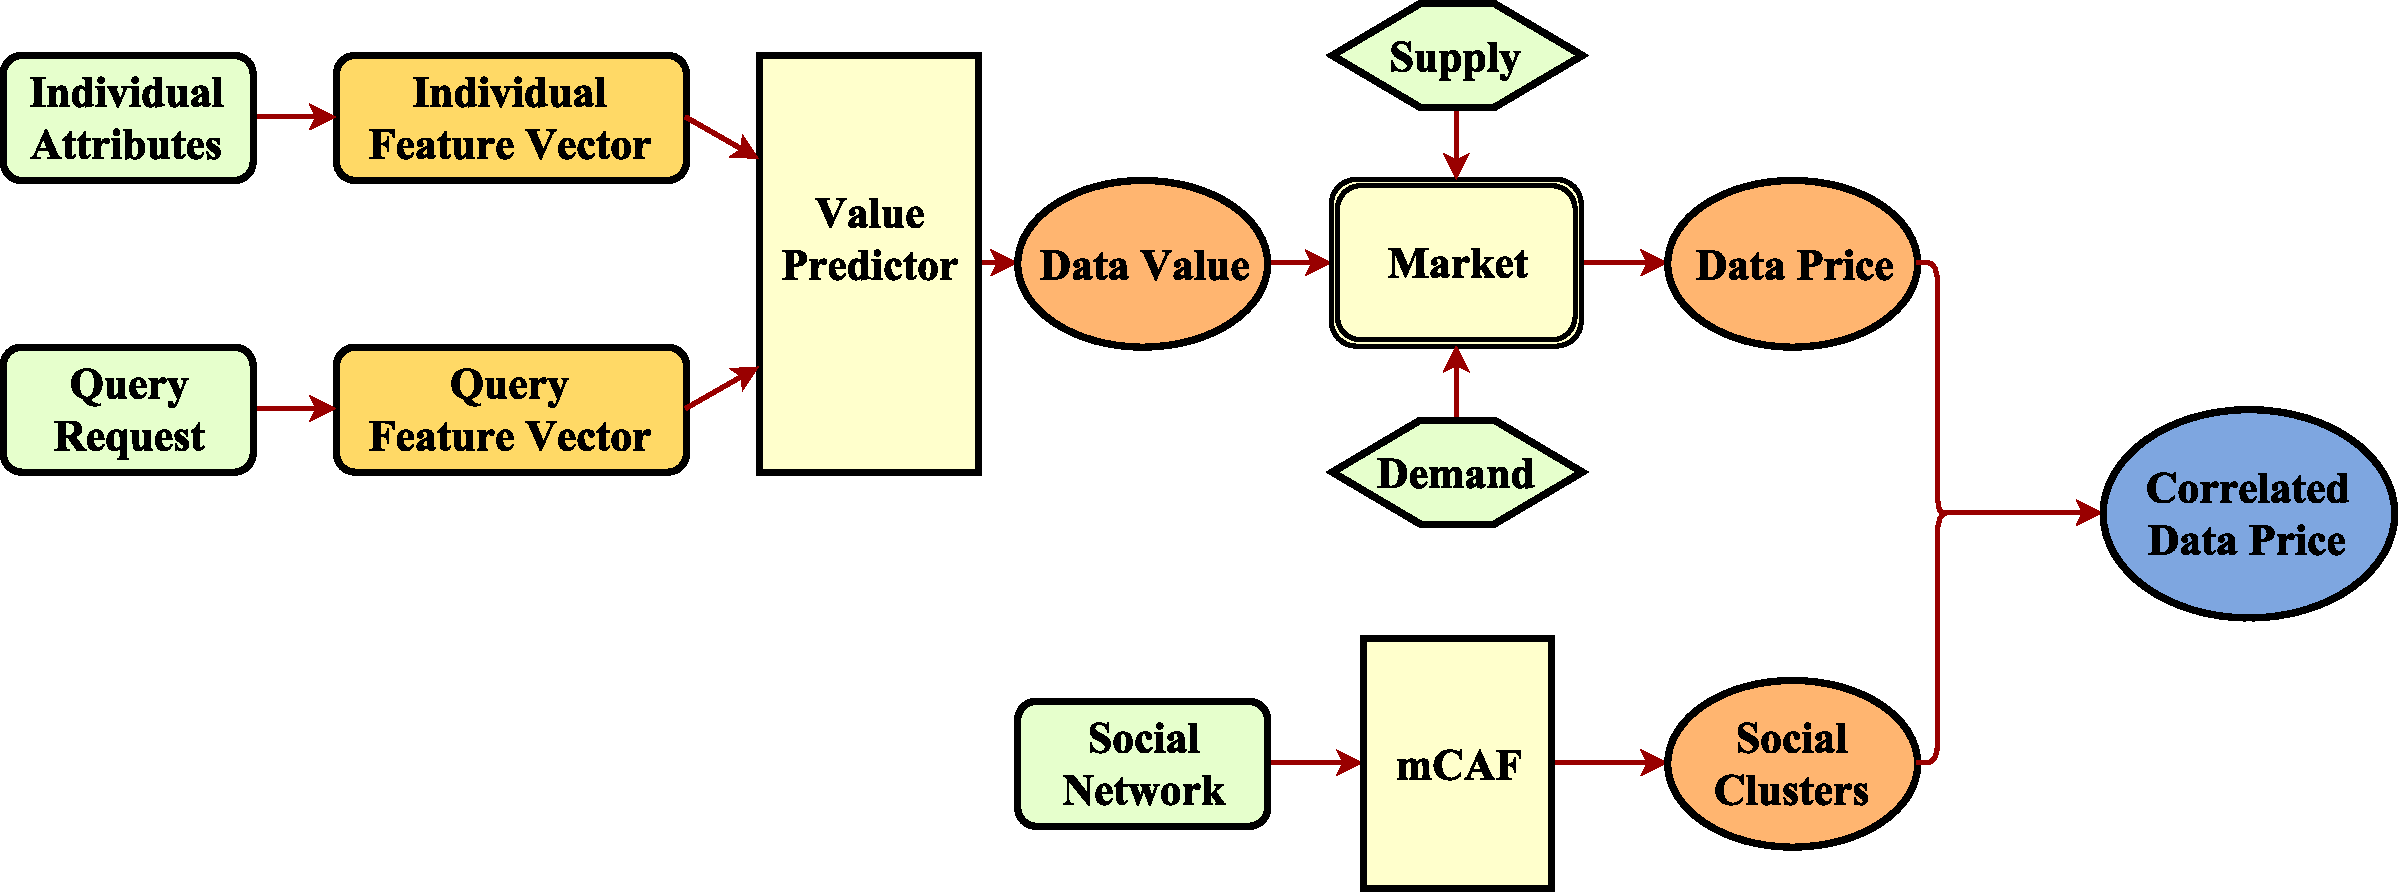
\includegraphics[width=0.8\textwidth]{fig/overview.pdf}
    \caption{The schematic illustration of the entire model}
    \label{fig:overview}
\end{figure}

\subsection{Vector-based Representation for Individuals and Queries}
\label{sec:vectors}

\subsubsection{Individual Feature Vectors}
\label{sec:individual_vec}

Based on the assumption in Sec.~\ref{sec:assumption} that private data can be classified into $m$ distinct categories, an individual's private data can thus be considered to consist of data records in multiple categories. In our model, we assume $m = 5$ and the categories include \emph{demographics}, \emph{family \& health}, \emph{property}, \emph{activities} and \emph{consumer} data.

The value of a person's entire data can then be split into $m$ independent \emph{category values}, the sum of which is equal to the original data value. Therefore, it makes sense to represent private information of individuals with an $m \times 1$ matrix, which is actually a vector:
\begin{equation}
    \sigma (I) = X = \left[\begin{matrix}
    X_1 & X_2 & \dots & X_m \\
    \end{matrix}\right]\text{,} \label{eqn:individual_feature_vector}
\end{equation}
where $I$ is a data provider, element $X_i (1 \leq i \leq m)$ in vector $X$ indicates the value of $I$'s data in the $i^{th}$ category, and function $\sigma(\cdot)$ extracts such category values based on life events and individual attributes. We define vector $X$ as person $I$'s \emph{feature vector} mainly because its elements reveals the essential value of $I$'s data that is distributed over $m$ categories.

The core part of Eqn.~\eqref{eqn:individual_feature_vector} is the function $\sigma(\cdot)$ that maps a person to the corresponding feature vector. The process is accomplished based on an analysis on the most influential factors of data value conducted by \emph{Financial Times} ~\cite{value_report}. The report points out that contrary to popular belief, the value of private information does not increase linearly with its amount. In fact, general information about a person, such as their age, gender and location is worth a mere \$0.0005 per person, or \$0.50 per 1,000 people. It is certain milestones in a person's life that prompt major changes in data values, such as becoming a new parent, moving homes, getting engaged, buying a car, or going through a divorce.

As is mentioned above, the value of data limited to a certain category is defined as the sum of potential risks and benefits incurred by it. On the basis of the Financial Times report, we develop a sophisticated model that implements the function $\sigma(\cdot)$. Here we briefly introduce its mechanism, the complete implementation can be referred to in Appx.~\ref{appx:sigma}

A person can possess a number of attributes at the same time, such as \emph{being engaged}, \emph{owning a home} and \emph{current job}, and some values of these attributes can possibly incur risks or benefits if known by a data company, for example, \emph{being engaged = true} and \emph{current job = government officer}. Our model includes a databases that stores the economical value vectors of certain attribute-value pairs, as is shown in Table~\ref{tab:database}, factors regarding to personal properties, health conditions and activities are considered more important and attached higher values than others.

\begin{table}[H]
    \centering
    \caption{Some of the most significant value vectors in our }
    \label{tab:database}
    \begin{tabularx}{0.8\textwidth}{X X}
\hline
\specialrule{0em}{2pt}{2pt}
    Attribute condition & Value vector / \$\\
\specialrule{0em}{2pt}{2pt}
\hline
\specialrule{0em}{2pt}{2pt}
	Being a millionaire & $\left[\begin{matrix} 0.116 & 0 & 0 & 0 & 0 \\ \end{matrix}\right]$\\
\specialrule{0em}{2pt}{2pt}
	Having a heart disease & $\left[\begin{matrix} 0 & 0.260 & 0 & 0 & 0 \\ \end{matrix}\right]$\\
\specialrule{0em}{2pt}{2pt}
	Registered at a real estate agency & $\left[\begin{matrix} 0 & 0 & 0.105 & 0 & 0 \\ \end{matrix}\right]$\\
\specialrule{0em}{2pt}{2pt}
	Interested in foreign travel & $\left[\begin{matrix} 0 & 0 & 0 & 0.135 & 0 \\ \end{matrix}\right]$\\
\specialrule{0em}{2pt}{2pt}
	Holding a store loyalty card & $\left[\begin{matrix} 0 & 0 & 0 & 0 & 0.136 \\ \end{matrix}\right]$\\
\specialrule{0em}{2pt}{2pt}
\hline
    \end{tabularx}
\end{table}
By significance we mean the magnitude of vectors calculated by norm $||X||$. Note that all our vectors concentrate values in one dimension (one data category), by which we intend to reduce data correlations between categories, which will be reconsidered in Sec.~\ref{sec:query_vec}.

\begin{minipage}[htbp]{0.9\textwidth}\centering
\begin{algorithm}[H]
	\SetKwInOut{Input}{Input}
	\SetKwInOut{Output}{Output}
	\caption{Feature vector extractor}\label{alg:sigma}
	\vspace{0.25\baselineskip}
	\Input{An individual $I$, information value database $\mathcal{S}$.}
	\Output{The feature vector $X = \sigma (P)$.}
	\BlankLine
	$X \leftarrow \left[\begin{matrix} 0 & 0 & \dots & 0 \\ \end{matrix}\right] $\;
	\For{$attr \in \{P\text{'s attributes}\}$}{
		\If{$\langle attr, P[attr]\rangle \in \mathcal{S}.values$}{
			$X \leftarrow X + \mathcal{S}[\langle attr, P[attr]\rangle]$\;
		}
	} 
	\Return X\;
\end{algorithm}
\BlankLine
\end{minipage}\\

As is shown in Alg.~\ref{alg:sigma}, our algorithm first sets the initial feature vector as an all-zero vector and then checks all the attributes of that person to determine if some attribute-value pairs can be found in our database. If a match is found, which means a certain value-creating condition is met, the value vector corresponding to that attribute-value pair will be added to the person's feature vector. In other words, a person's feature vector is the sum of all value vectors of the conditions satisfied by his personal attributes.



Based on Alg.~\ref{alg:sigma}, we are able to determine the typical individual feature vectors of various social subgroups, which will be discussed in Sec.~\ref{sec:task1}.


\subsubsection{Query Feature Vector \& Correlation Matrix}
\label{sec:query_vec}

Similar to \emph{individual feature vectors} defined in Sec.~\ref{sec:individual_vec}, we define an $m \times 1$ \emph{query feature vector} $Y = \varphi(q)$ that represents the query request $q$ with $m$ scalars, each stands for the intensity of private data requested in an data category. The intensity is measured by the amount as well as accuracy of requested data. For instance, if full information of a person's demographic characteristics and purchasing history is requested, the query feature vector should be $\left[\begin{matrix} 1 & 0 & 0 & 0 & 1 \\ \end{matrix}\right]$. 

However, with merely query vectors we are still not able to accurately calculate the value of private information, as data correlations tend to occur between different categories of data. To address this phenomenon, we introduce a \emph{correlation matrix} $C$ that takes connections between various categories of data into consideration, and define that the value of a piece of data record from individual $I$ queried with feature vector $Y$ as
\begin{equation}
    v = \sigma (P) C Y^T \label{eqn:value}
\end{equation}

Ideally, with no data correlations the correlation matrix $C = E = diag\left(\left[\begin{matrix} 1 & 1 & \dots & 1 \\ \end{matrix}\right]\right)$. In order to estimate the intensity of data correlations, we fill the correlation matrix $C$ in following manners:
\begin{equation}
    C_{i, j} = \left|cov(c_i, c_j)\right|
\end{equation}
where $c_i$ and $c_j$ are the $i^{th}$ and $j^{th}$ data category value. Our final correlation matrix $C$ is computed based on feature vectors extracted from typical population subgroups, which will be discussed in detail in Sec. \ref{sec:task1} and demonstrated in Fig.~\ref{fig:fvs}.
\begin{equation}
    C = \left[\begin{matrix} 1.0000 & 0.6463 & 0.8443 & 0.8231 & 0.2793 \\
    0.6463 & 1.0000 & 0.6767 & 0.2197 & 0.2226 \\
    0.8443 & 0.6767 & 1.0000 & 0.5403 & 0.1649 \\
    0.8231 & 0.2197 & 0.5403 & 1.0000 & 0.6916 \\
    0.2793 & 0.2226 & 0.1649 & 0.6916 & 1.0000 \\ \end{matrix}\right] \label{eqn:C}
\end{equation}
which suggests that the most magnificent data correlations exists between data categories of
\begin{itemize}
\item Demographics \& Property
\item Demographics \& Activities
\item Activities \& Consumer
\end{itemize}

On the basis of Eqn.~\eqref{eqn:value} and Eqn.~\eqref{eqn:C}, we are able to calculate the raw value of a specific data record and its query requests. However, there remain external factors that have strongly affect the real value of private data, among which the most significant one is time. It is widely acknowledged that data value decays with time. On the other hand, a consistent data record sequence collected throughout a long time period should be attached additional value. Similarly, data scale affects the value of private data nonlinearly. Thus, an amendment is made with Eqn.~\eqref{eqn:value} by introducing variations:
\begin{equation}
    v' = e^{\omega T - \tau t} N^{\mu} v\label{eqn:amend}
\end{equation}
where the dynamic element $T$ denotes the sequence length ($/ days$) of data, $t$ stands for the freshness of private data (days since the data is generated), and $N$ represents the number of data records. Parameters $\omega, \tau$ and $\mu$ affects the real value in exponential and multinomial manners. In our estimation based on information rules~\cite{shapiro1998information}, $\omega = 1.28 \times 10^{-3}, \tau = 9.50\times 10^{-4} \text{ and } \mu = 1.05$. 

\subsection{Dynamic Market System \& Pricing Strategy}
\subsubsection{PI Demand Model}
The demand $d_i$ for the private data is originate from the individual $i$ (who themselves might posses the data or can generate the data). The availability of $d_i$ to the demander $j$ is captured by a matrix $\mathcal{M}$: the larger $\mathcal{M}_{i,j}$, the larger a fraction of $i$ will be demanded by $j$. Specially, the demand that $j\in J^+$ will see from $i$ is $d_i\cdot\frac{\mathcal{M}_{i,j}}{\sum_{\omega\in J^+}P_{i,\omega}}$. The matrix $\mathcal{M}$ will in practice depend on time latencies, as well as political and cultural issues. It need not be symmetric. For the purpose of the general model, we are agnostic to the derivation of $\mathcal{M}$. An individual $j\in J^+$  will incur a risk of $r_j$ per unit of demand; This risk is the result of data breach/leakage, which will bring some potential trouble to the person or the related business.  To encourage individuals to provide the PI, the buyer offers payments $P_i$ to the person $i$. These payments are different from person to person, and can be derived from the domains (e.g. social media, financial transactions, and health/medical records) and some properties of that person.

Different people have different tradeoffs between the price and risk of PI. We model this fact by assuming that each person $j$ has a trade off factor $\lambda_j$ that describes the risk-to-benefit ratio of PI. We use Benefit-Divide-Risk Analysis (BDRA) to calculate $\lambda_j$. It is defined in Eqn.~\eqref{eqn:risk to benefit}, where $s_{benefit}$ and $s_{risk}$ are benefit score and risk score. Benefit score is the data value we have calculated. Risk score is calculated in Table~\ref{tab:score}. 

\begin{equation}\label{eqn:risk to benefit}
    \lambda_j=\frac{s_{benefit}}{s_{benefit}+s_{risk}},
   \lambda_j \in [0,1]
\end{equation}

\begin{table}[!htb]
    \centering
    \caption{ Calculation of risk score (1,2,3,4,5 stand for level of risk)}
    \label{tab:score}

    \begin{tabularx}{\textwidth}{c X X X X X }
\hline
\specialrule{0em}{2pt}{2pt}
    Criterion & 1 & 2 & 3 & 4 & 5\\
\specialrule{0em}{2pt}{2pt}
\hline
\specialrule{0em}{2pt}{2pt}
Financial Risk  & 0.05 & 0.062 & 0.074 & 0.09 & 0.128 \\
\specialrule{0em}{2pt}{2pt}
Health Risk   & 0.06 & 0.09 & 0.11 & 0.14 & 0.24  \\
\specialrule{0em}{2pt}{2pt}
Family Risk   & 0.05 & 0.062 & 0.088 & 0.15 & 0.22  \\
\specialrule{0em}{2pt}{2pt}
Social Risk   & 0.03 & 0.062 & 0.1 & 0.13 & 0.17  \\
\specialrule{0em}{2pt}{2pt}
\specialrule{0em}{2pt}{2pt}
\hline
    \end{tabularx}
\end{table}
   
Thus, the \emph{demanding} of an individual $j\in J^+$ is
\begin{equation}\label{equ:demand model}
D(j) = \lambda_j P_j-r_j\sum_i\frac{d_i \mathcal{M}_{i,j}}{\sum_{\omega\in J^+}\mathcal{M}_{i,\omega}},
\end{equation}

\paragraph{Asymmetric Information.} This part illustrates that purchasers possess a substantial amount of information about data providers. These facts suggest that the restrictions such as policy and culture - which make it difficult for data providers to adjust prices when they provide private information to purchasers over time - have different price effects across different sellers and buyers depending on their privately revealed types, cultural and political issues. Incorporating such factors in our model therefore become important in anticipation of using the model to study the PI problem.
Formally, we estimate these effects in the following equation~\ref{equ:default},
\begin{equation}\label{equ:default}
Default_{i,t}=\alpha_{j(i)}+\alpha_t+\sum_{n=1}^{5}\beta_n1_{\psi_i,t=n}+\epsilon_{it}
\end{equation}
Here the dependent variable is an indicator for any instance of default by purchaser $i$ after period $t$, and the key coefficients $\beta_n$ capture differences in default rate across different private information, which denoted by $\psi$. Meanwhile the fixed effects for purchaser $i$ and time $t$ help ensure that these risk comparisons are made within otherwise observably similar purchasers.

\paragraph{Model Exposition} This section presents the PI model. The backbone of the demand model is a finite mixture of agency types, each of whom has demand over PI providers.

Our model denotes type by $\theta$. We specify several parameters to be estimated for each type. First, each type enjoys a flow utility $d_{j\theta}$ from buying from person $j$ and a time utility $n_{j\theta}$ from transacting with person $j$; meanwhile the utility is normalized to zero. Additionally, in order to capture the adjustment cost, each type pays a agency cost $s_{j\theta}$ for refer to potential related PI with person $j$. The parameters $\{d_{j\theta}, n_{j\theta}, s_{j\theta}\}_{(\theta,j)\in\Theta\times J}$ are the key demand parameters to be estimated in the model, along with a probability distribution $\mu_\theta$ over types.

Integrating over taste shocks $\epsilon$ for each choice yields the standard Bellman equation for continuation values $V$, which is shown in Eqn.~\eqref{eqn:Vbe}.
\begin{equation}
V(\theta,j,k)=\log\left(\sum_{j',k'}\exp(v(j',k'|j,k,\theta))\right),\label{eqn:Vbe}
\end{equation}
where the lower-case $v$ term denotes total expected payoffs. The value of $v$ depends on data buyers' past-period and current-period choices. The expectation $\mathbb{E}_\theta$ can be decomposed as Eqn.~\eqref{equ:e},
\begin{equation}\label{equ:e}
\mathbb{E}_\theta[V(\theta',j,b)]=(1-\delta(\theta))T_{\theta\theta'}(\theta)V(\theta',j,b)+\delta(\theta)T_{\theta\theta'}(\theta)V(\theta'',0,0).
\end{equation}

With the establishment of Eqn.~\eqref{eqn:amend}, our model further takes time variations and scale effects as dynamic elements into consideration to estimate the worth of personal data over time.

% \begin{table}
%     \centering
%     \caption{$\gamma$ Corresponding to the Domains of Private Data}
%     \label{tab:priceReg}
%     \begin{tabular}{c c}
% \hline
% \specialrule{0em}{2pt}{2pt}
%     	Denotation & Types of Agencies\\
% \specialrule{0em}{2pt}{2pt}
% \hline
% \specialrule{0em}{2pt}{2pt}
% 	$\gamma_1=0.1$ & Personal Data, e.g. name, address, picture, etc.\\
% \specialrule{0em}{2pt}{2pt}
% 	$\gamma_2=0.2$ & Transaction Data, e.g. on-line purchases, search history, etc.\\
% \specialrule{0em}{2pt}{2pt}
% 	$\gamma_3=0.3$ & Social Media Data, e.g. post, picture etc.\\
% \specialrule{0em}{2pt}{2pt}
% \hline
%     \end{tabular}
% \end{table}

% \subsubsection{Dynamic Element}
% Our model introduces a variation $\gamma$ as a dynamic element to illustrate the worth of personal data over time. There are several domains of private data, e.g. personal data (such as name, address, picture), transaction data (e.g. on-line purchases, search history), and social media data (e.g. posts, picture).
% \begin{equation}
% p_{dynamic} = \frac{p}{e^{\gamma t}}
% \end{equation}
% Since the degradation rate varies from different domains of data. Information such as social media data is more time-sensitive to information such as name, address. The different domains of private data has different value of $\gamma$, shown as Table~\ref{tab:dynamic}.

% \begin{table}
%     \centering
%     \caption{$\gamma$ Corresponding to the Domains of Private Data}
%     \label{tab:dynamic}
%     \begin{tabular}{c c}
% \hline
% \specialrule{0em}{2pt}{2pt}
%     	Denotation & Types of Agencies\\
% \specialrule{0em}{2pt}{2pt}
% \hline
% \specialrule{0em}{2pt}{2pt}
% 	$\gamma_1=0.1$ & Personal Data, e.g. name, address, picture, etc.\\
% \specialrule{0em}{2pt}{2pt}
% 	$\gamma_2=0.2$ & Transaction Data, e.g. on-line purchases, search history, etc.\\
% \specialrule{0em}{2pt}{2pt}
% 	$\gamma_3=0.3$ & Social Media Data, e.g. post, picture etc.\\
% \specialrule{0em}{2pt}{2pt}
% \hline
%     \end{tabular}
% \end{table}
\subsubsection{Buyer-Seller Relationship Influence to Price}

% \begin{figure}[htbp]

% \end{figure}

As Fig.~\ref{fig:ad_rev} shows, internet advertising revenue has grown strongly over the last ten years. In 2013 it hit \$42.8 billion in the US. Internet giants such as Google and Facebook have business models underlined by the use of personal data, but most people would have trouble knowing who exactly has access to the data trail they are generating across the internet \cite{Detemple2016The}.  A recent study by JPMorgan Chase \cite{brustein2012start} found that each unique user is worth approximately \$4 to Facebook and \$24 to Google. 

\begin{wrapfigure}[16]{r}{0.65\textwidth}
	\vspace{-1.8\baselineskip}
	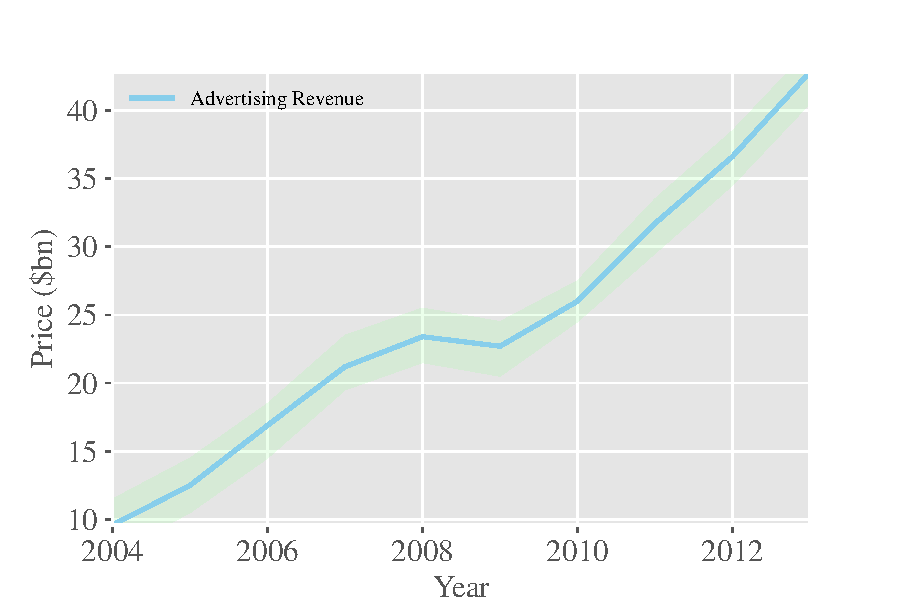
\includegraphics[width=\linewidth]{fig/adv_rev.pdf}
	\vspace{-1.5\baselineskip}
	\caption{US Internet Advertising Revenue by Year, the shadow represents statistical uncertainty and variance.}
	\label{fig:ad_rev}
\end{wrapfigure}

Besides commercial corporations, there are also other agencies who purchase PI. Mozilla collect data about users to better personalize their experiences with their open source products such as Firefox, Thunderbird. The information they gather through analytics can be used to make their product easier to use. They also use cookies (small data files placed in browsers) to remember language preferences. Center for Disease Control utilizes the data shared to trace the spread of disease in order to prevent further outbreak.

There are $3$ types of agencies in our model and their purchasing power is shown as Table~\ref{tab:task_3}. The price estimation system concerning with different agencies who purchased the PI is illustrated as Eqn.~\eqref{equ:agency}.
\begin{table}
    \centering
    \caption{Purchasing power of three types of agencies}
    \label{tab:task_3}
    \begin{tabular}{c c}
\hline
\specialrule{0em}{2pt}{2pt}
    	Denotation & Types of Agencies\\
\specialrule{0em}{2pt}{2pt}
\hline
\specialrule{0em}{2pt}{2pt}
	$\mathcal{Q}_1$ & Commercial Corporation, e.g. Google, Facebook, Microsoft, etc.\\
\specialrule{0em}{2pt}{2pt}
	$\mathcal{Q}_2$ & Non-Profit Organization (NPO), e.g. Mozilla, GNU, WWF, etc.\\
\specialrule{0em}{2pt}{2pt}
	$\mathcal{Q}_3$ & Government Department, e.g. NSA, Department of Energy, etc.\\
\specialrule{0em}{2pt}{2pt}
\hline
    \end{tabular}
\end{table}

\begin{equation}\label{equ:agency}
P_{agency}=\sum_{j=1}^{M}\tau_j\mathcal{Q}_i,
\end{equation}
where $\tau_j$ is the control level of individual $j$ to sell his/her own data, there are totally $M$ individuals in a group/nation, $\mathcal{Q}_i$ can be $\mathcal{Q}_1, \mathcal{Q}_2$ or $\mathcal{Q}_3$ which represents the purchasing power of different types of agencies.
% \subsection{Clustered social network}
\subsection{\emph{mCAF}: a Multi-dimensional Clustering Algorithm for Friends of Social Network Services}
The multi-dimensional clustering algorithm for friends (\emph{mCAF}) is adopted by us to perform multi-dimensional clustering. Multi-dimensional clustering algorithms on social networks are progressively gaining popularity due to the information and insights produced using large-scale social data. ~\cite{khobzi2014significant} describes the user's opinions, comments, and likes in social media have significant relationships with the popularity of that post. Multi-dimensional cluster analysis is a strategy for identifying different Facebook users' fan groups and provides insights to prompt further research analytics \cite{wallace2014likes}. Both network structures and profile information should be taken into consideration while analyzing a user's clusters on social networks \cite{gross2005information,mcauley2014discovering}. 

In this study, we used the Facebook Graph API to retrieve information of 600 users. First, we define the measurements of clustering.

\paragraph{Social Circles.} A social circle is a group of people who have the same interests or join the same activity. We define $M_{ij}$ as the number of mutual friends of user $i$ and $j$ and $G_{ij}$ as the interaction value. We quantify the subject's interactions within the community to obtain $S_{ij}$ with Eqn.~\eqref{equ:mg} and then normalize the result as Eqn.~\eqref{equ:s_ij}
\begin{equation}\label{equ:mg}
MG_{ij}=M_{ij}+G_{ij}, \mathbb{MG}=\{MG_{xy}\mid x, y\in1,2,3,\dots,n\}
\end{equation}
\begin{equation}\label{equ:s_ij}
S_{ij}=\frac{MG_{ij}}{\max(MG)}, \mathbb{S}=\{S_{xy}\mid x,y\in 1,2,3,\dots, n\}
\end{equation}

\paragraph{Regions.} We determine the region of the users and then calculate the distances between them and store them as a dataset described by $\{D_1, D_2, D_3, D_4\}$. Take the calculation of distance between $A$ and $B$ as an example, $D_1$ represents the distance between the hometowns of $A$ and $B$; $D_2$ represents the distance between the current residence of $A$ and $B$; $D_3$ represents the distance between $A$'s hometown and $B$'s current residence; $D_4$ represents the distance between $A$'s current residence and $B$'s hometown. The calculation of $R_{ij}$ is shown as Eqn.~\eqref{equ:r_ij}.
\begin{equation}\label{equ:r_ij}
R_{ij}=\alpha \times D_1 + \beta\times D_2+\gamma\times D_3+\delta\times D_4
\end{equation} 

\paragraph{Organizations.} If two individuals attended the same school or worked in the same company, the organizations measurement $O_{ij}$ is set equal to 1 since they have a connection. If no connection is present, the $O_{ij}$ is set equal to 0.

\paragraph{Tie strength.} 
We retrieve related information and use the method described in \cite{treeit2014tsai} to calculate the tie strength as $T_j$, which indicates the tie strength between a user and his $j$th friend.

\emph{mCAF} maps a user's friends into un-directed, weighted graphs. We define the entire graph as $G=\{V,E\}$, in which $V$ is the set of vertices and $E$ is the set of edges, defined as $\left\{E_{i,j}(e_{i,j}^k)\right\}$, which represents a connection if a value $e_{i,j}^k$ is greater than zero between nodes $i$ and $j$ under measurement $k$.

\paragraph{Definition of vertex structure.} Let vertex $i\in V$, where the structure of $i$ is defined by its neighborhood denoted by $\varGamma(i)$ in Eqn.~\eqref{equ:varGamma}

\begin{equation}\label{equ:varGamma}
\varGamma(i)=\{j\mid j\in V \wedge E_{i,j} \in E \}
\end{equation}

\paragraph{Definition of the weight summary of one measurement to one node} Eqn.~\eqref{weight} defines the summary values of measurements from vertex $j$, which is connected to $i$:
\begin{equation}\label{weight}
W_i^k=\sum_{j=1}^{j=|V|}(e_{i,j}^k), where j\in \varGamma(i)
\end{equation}

\paragraph{Definition of the weight summary of one measurement to two nodes}
Let vertex $m \in V$, and let edges from $(i, m)$ and $(j, m)$ exist. Eqn.~\eqref{equ:T_ij} defines the summary values of measurements from vertex $m$, which is connected to $i$ and $j$:

\begin{equation}\label{equ:T_ij}
T_{i,j}^k=\sum_{m=1}^{m=|V|}(e_{i,m}^k+e_{j,m}^k)\ where\ m\ \in \varGamma(i)\ and\ m \in \varGamma(j)
\end{equation}

\begin{minipage}[t]{0.9\textwidth}\centering
\begin{algorithm}[H]
	\SetKwInOut{Input}{Input}
	\SetKwInOut{Output}{Output}
	\caption{Multi-dimensional clustering algorithm(\emph{mCAF})}\label{alg:mcaf}
	\vspace{0.25\baselineskip}
	\Input{$G=\{V,E\}, \{\epsilon^k\}, \{\mu^k\}$}
	\Output{Clustering result}
	\BlankLine
	$count^1=0; count^2=0;count^3=0;k^1=0;k^2=0;k^3=0;$
	
	\ForEach{ vertex $i\in V$}{
		\For{each vertex $j\in \varGamma(i)$}
		{
		\If {$(S_{i,j}^k\times\mu^k$ has max value where $k=1\sim3$ and $j\in N_{\epsilon^k}(i)$}
		{$count^k=count^k+1;$}
		}
		Set(|$count^1$|, $|count^2|$, $|count^3|$) as ($k_1, k_2, k_3$);
		
		\eIf{$k^a$ has only one max value}{$k_{max}(i)=a$;}
		{label $i$ as uncertain $V$;}
	}
	\ForEach{ unstagged vertex $p\in V$}{
	\If{$q\in N_{\epsilon^{k_{max(p)}}}(p)$}{
	\If{first $q$}{
	generate new clusterID;
	
	insert $q$ into queue $Q$;}
	\While{$Q\neq0$}{
	q=dequeue(Q);
	
	\ForEach{ $r\in N_{\epsilon^{k_{max(p)}}}(q)$}{
	\If{($r$ is untagged)}{
	insert $r$ into queue $Q$;
	
	assign current clusterID to $r$;}}
	remove $q$ from $Q$;
	}}}
\end{algorithm}
\BlankLine
\end{minipage}\\

\paragraph{Definition of structure similarity} She structure similarity of two vertices $i$ and $j$ is defined as Eqn.~\eqref{equ:Sim}:
\begin{equation}\label{equ:Sim}
Sim_{i,j}=\left\{S_{i,j}^1, S_{i,j}^2, S_{i,j}^3\right\}=\frac{\{T_{i,j}^1, T_{i,j}^2, T_{i,j}^3\}}{\sqrt{W_i^1\cdot W_j^1+W_i^2\cdot W_j^2+W_i^3\cdot W_j^3}}
\end{equation}

\paragraph{Definition of the threshold neighbor} If two nodes can be clustered together based on measurement $k$, their structure similarity value $S^k_{i,j}$ must be greater than the preset threshold $\epsilon^k$ to filter out noise. Eqn~\eqref{equ:N} defines neighbors with qualified similarity structure values. The parameter $\epsilon^k$ could be estimated via training. 

\begin{equation}\label{equ:N}
N_{\epsilon^k}(i)=\left\{j|j\in \varGamma(i) \wedge S_{i,j}^k \leq \epsilon^k \right\}\ where\ k=1\ to\ 3
\end{equation}

The complete mCAF algorithm is described in Algorithm~\ref{alg:mcaf}.

The clustering result of \emph{mCAF} is shown in Fig.~\ref{fig:mcaf}. The social network of several individuals are clustered into 8 subgroups. The visualization of network shows the correlations between different people.

\begin{figure}[!htb]
\begin{minipage}[t]{0.48\textwidth}
	\begin{center}
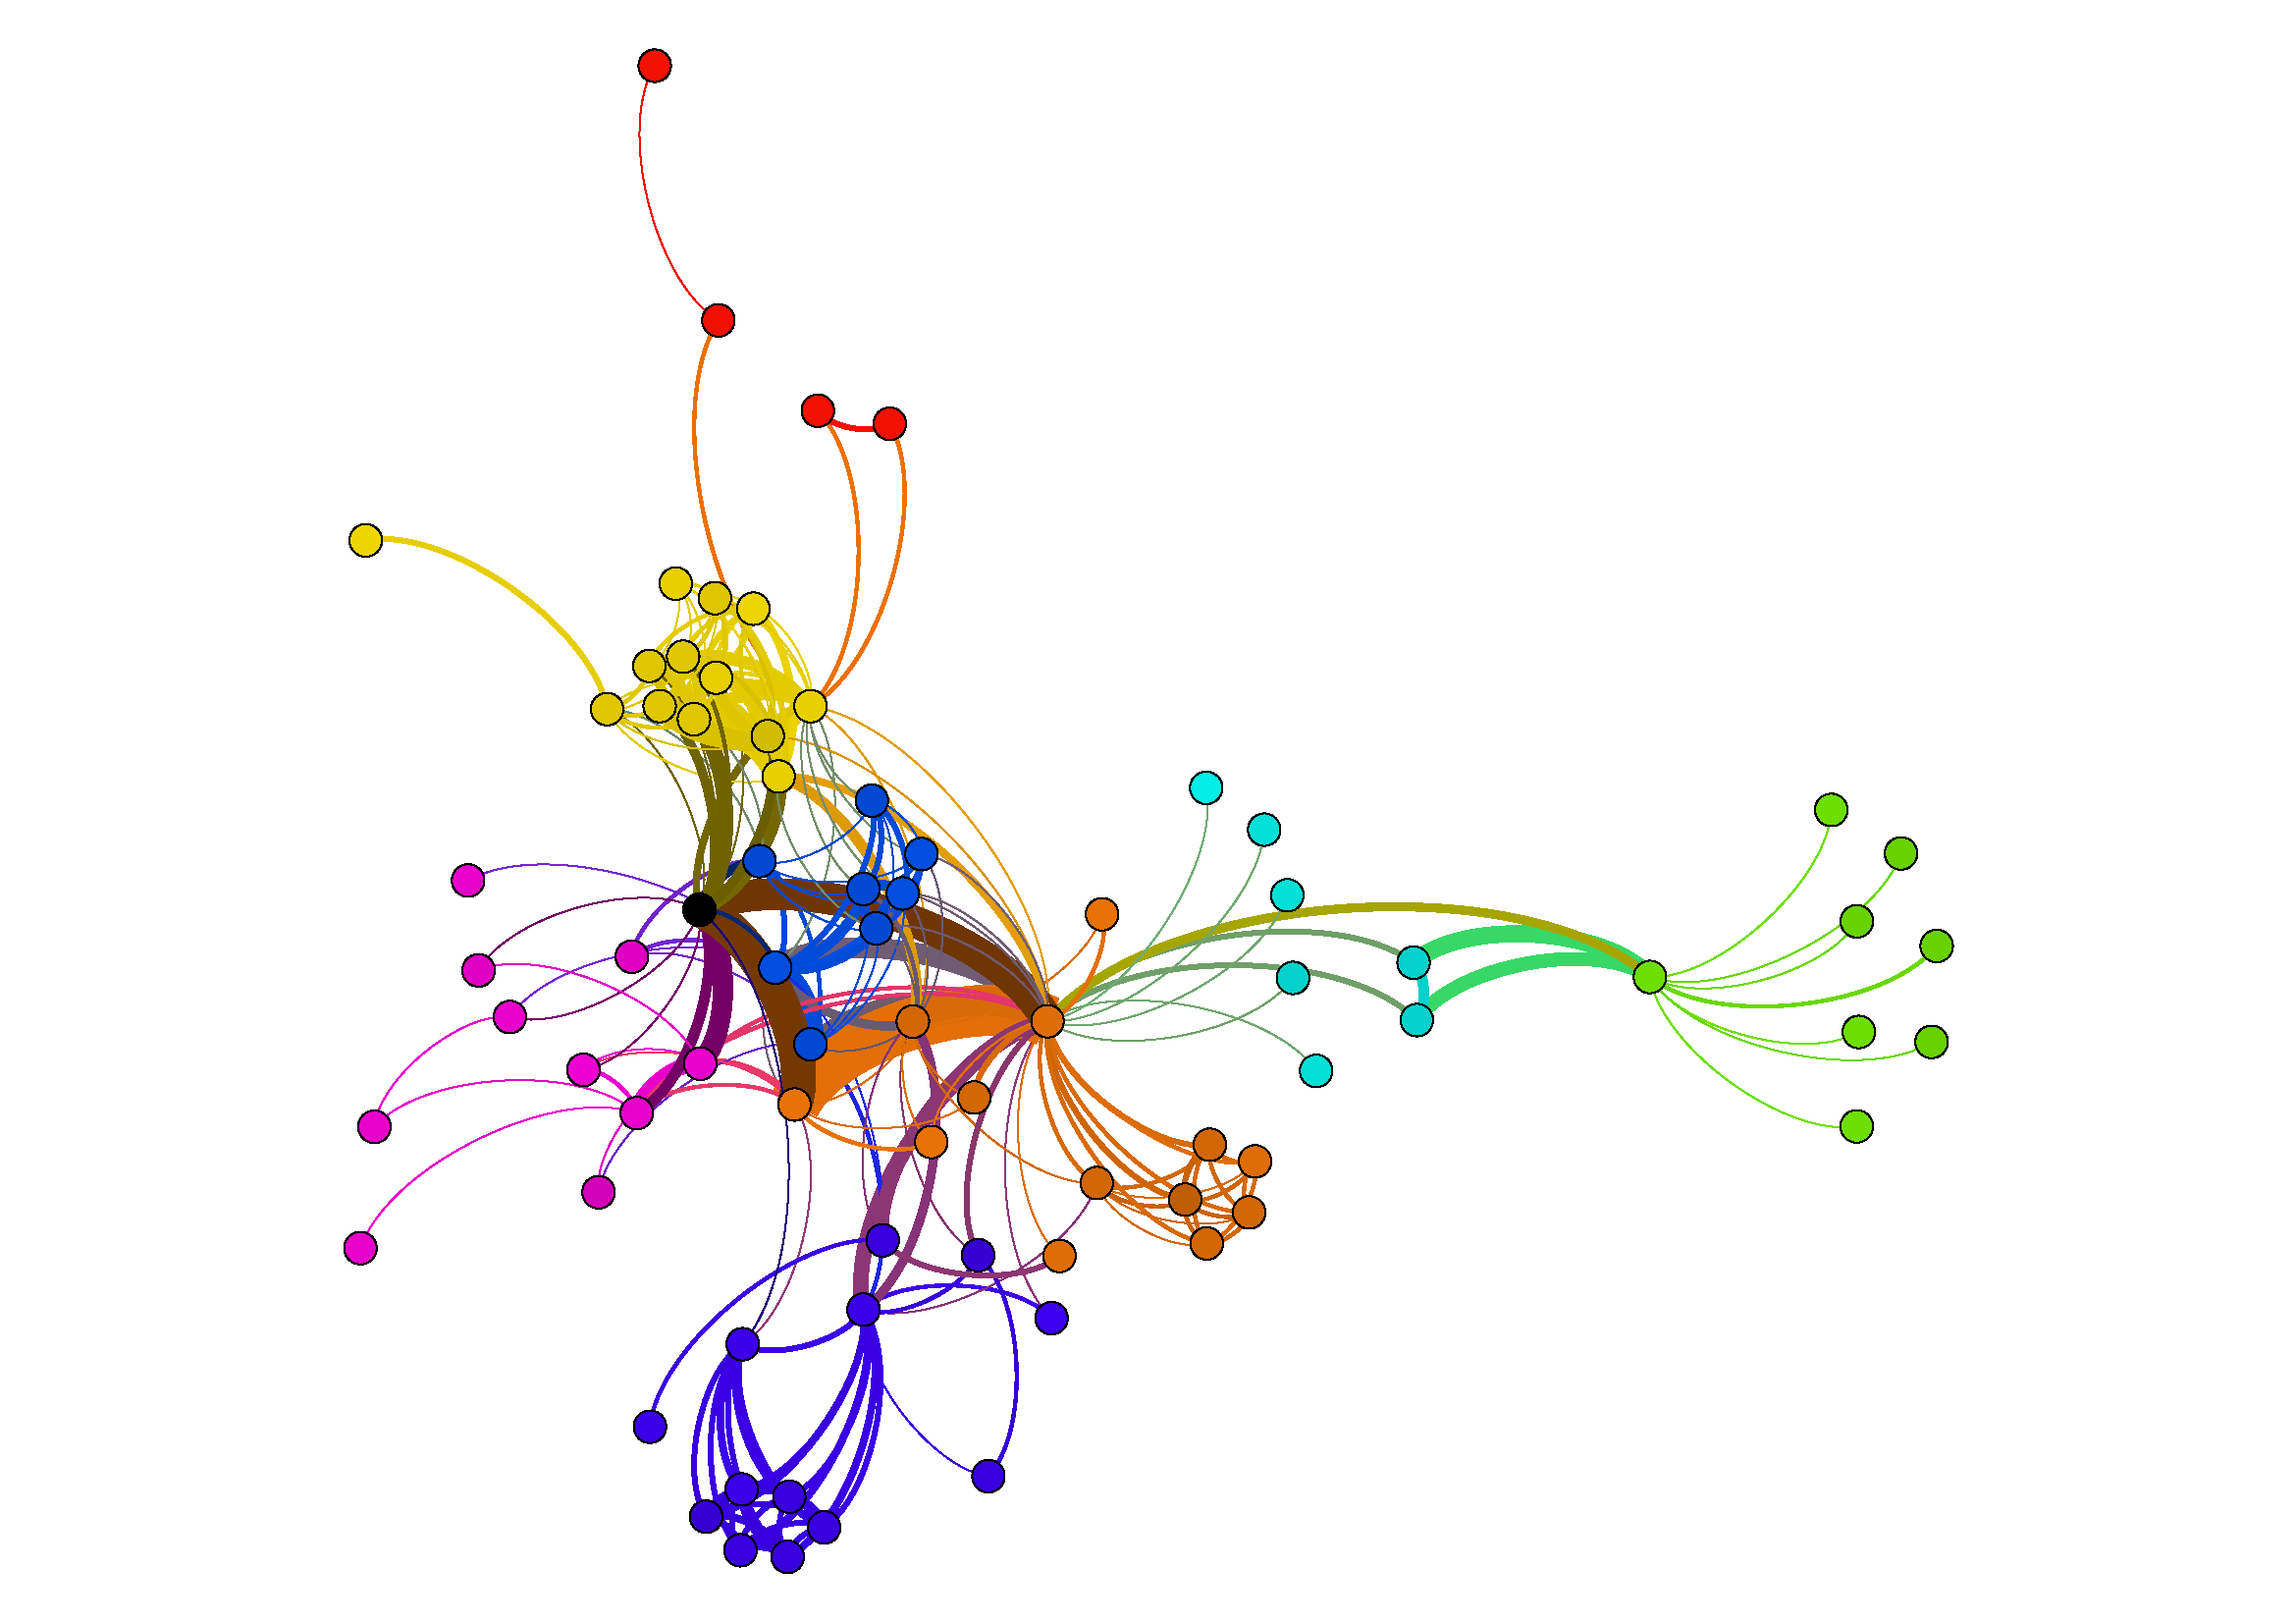
\includegraphics[width=\linewidth]{fig/cluster.png}
\caption{\emph{mCAF} Clustering Result of Social Network}
\label{fig:mcaf}
\end{center}
\end{minipage}
\hspace{0.04\textwidth}
\begin{minipage}[t]{0.48\textwidth}
\begin{center}
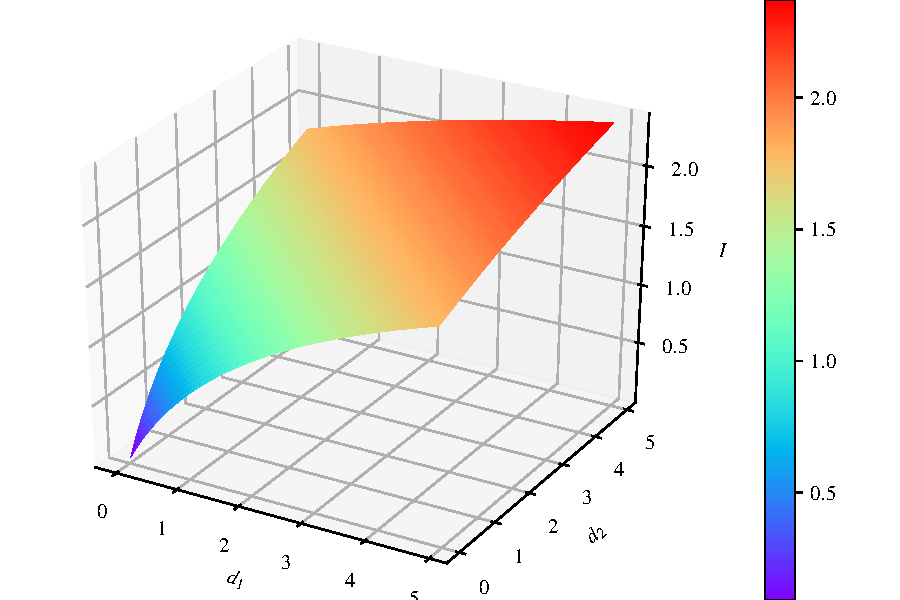
\includegraphics[width=\linewidth]{fig/network_effect.pdf}
\caption{Relationship between data size $d_i$ and information $\mathcal{I}$}
\label{fig:dI}
\end{center}
\end{minipage}
\end{figure}


To better evaluate the network effects of data sharing, we investigate the relationship between two individuals who are highly linked and discover the relationship between the data size from one person and the information it can provide. Define $d_i$ is the data size from person $i$ and $\mathcal{I}=f(d)\in [0,1]$ represents the information the data on one person can provide. There are totally $M$ individuals. Eqn.~\eqref{equ:dI} represents the function between $d$ and $\mathcal{I}$ and Fig.~\ref{fig:dI} illustrates the function in the circumstance of $i=2$.
\begin{equation}\label{equ:dI}
\mathcal{I}=\log(1+\sum_{i=1}^{M}d_i)
\end{equation}


\section{Experimental Results}
\label{sec:experiments}

\subsection{Task 1: Price Point for Protecting One's Privacy and PI in Various Applications}
\label{sec:task1}
In order to accurately model risk to account for both 1) characteristics of the individuals, and 2) characteristics of the specific domain of information, we introduce the concept of individual and query feature vectors discussed in Sec.~\ref{sec:vectors}. 

\begin{figure}[!htbp]
    \centering
    \subfigure[Age Distribution]{
        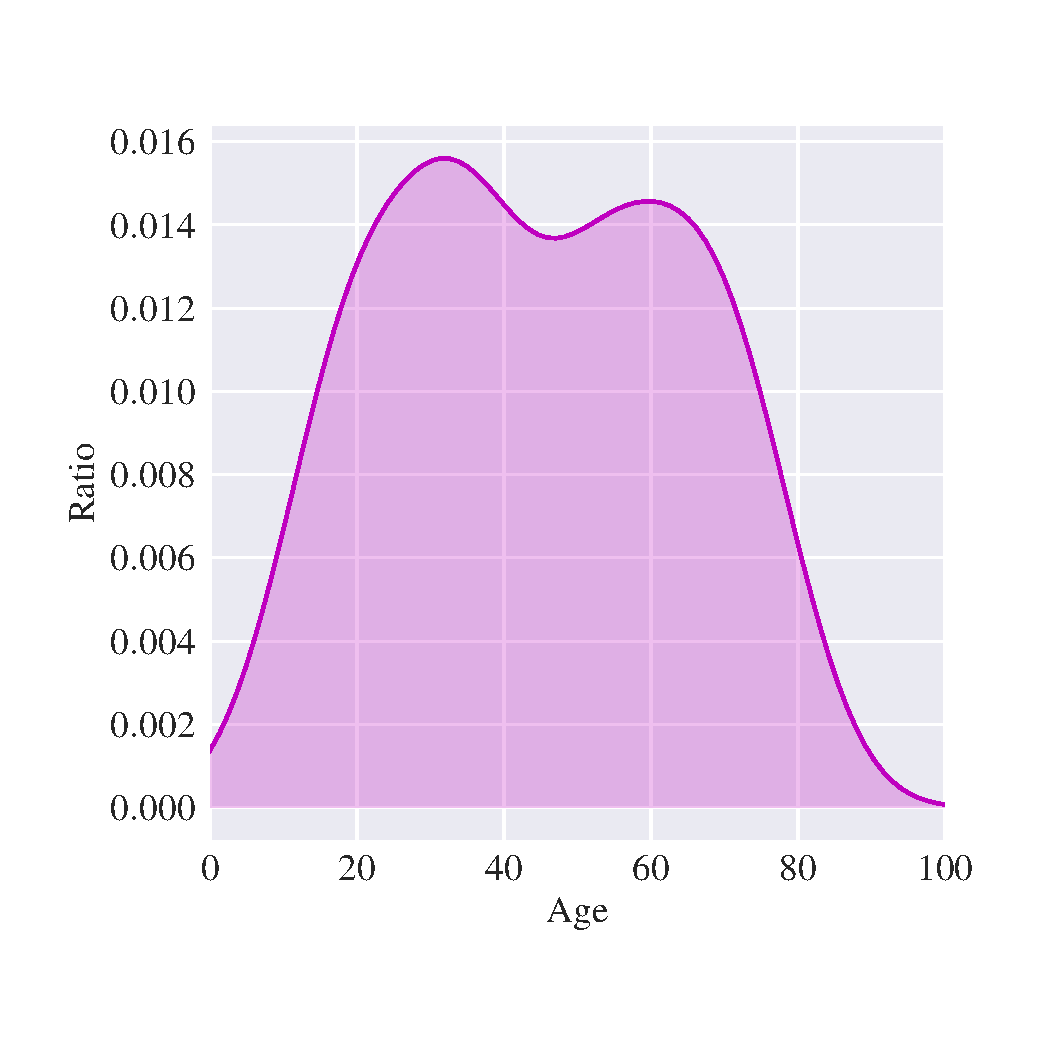
\includegraphics[width=0.31\textwidth]{fig/age.pdf}
        \label{fig:age_distribution}
    }
    \subfigure[Gender Distribution]{
        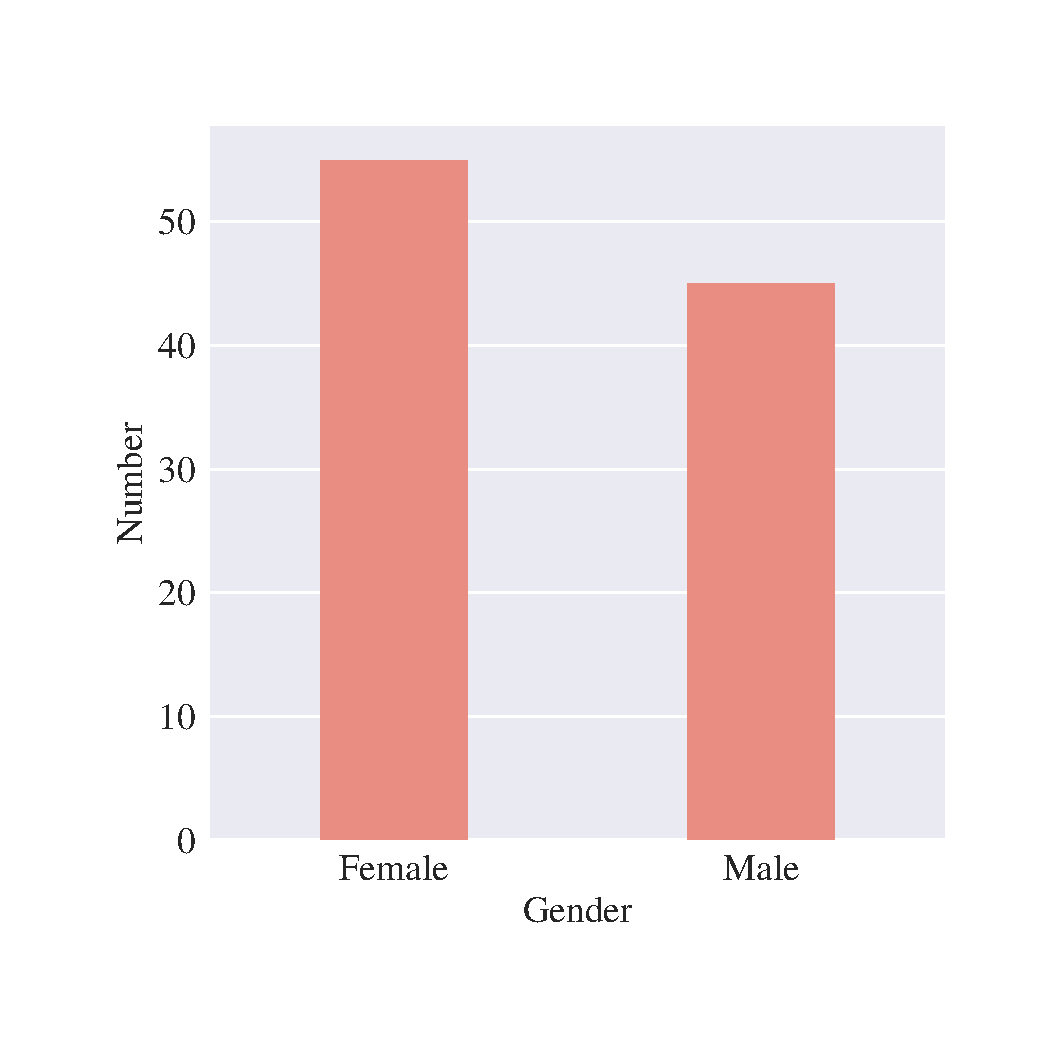
\includegraphics[width=0.31\textwidth]{fig/gender.pdf}
        \label{fig:gender_distribution}
    }
    \subfigure[Occupation Distribution]{
        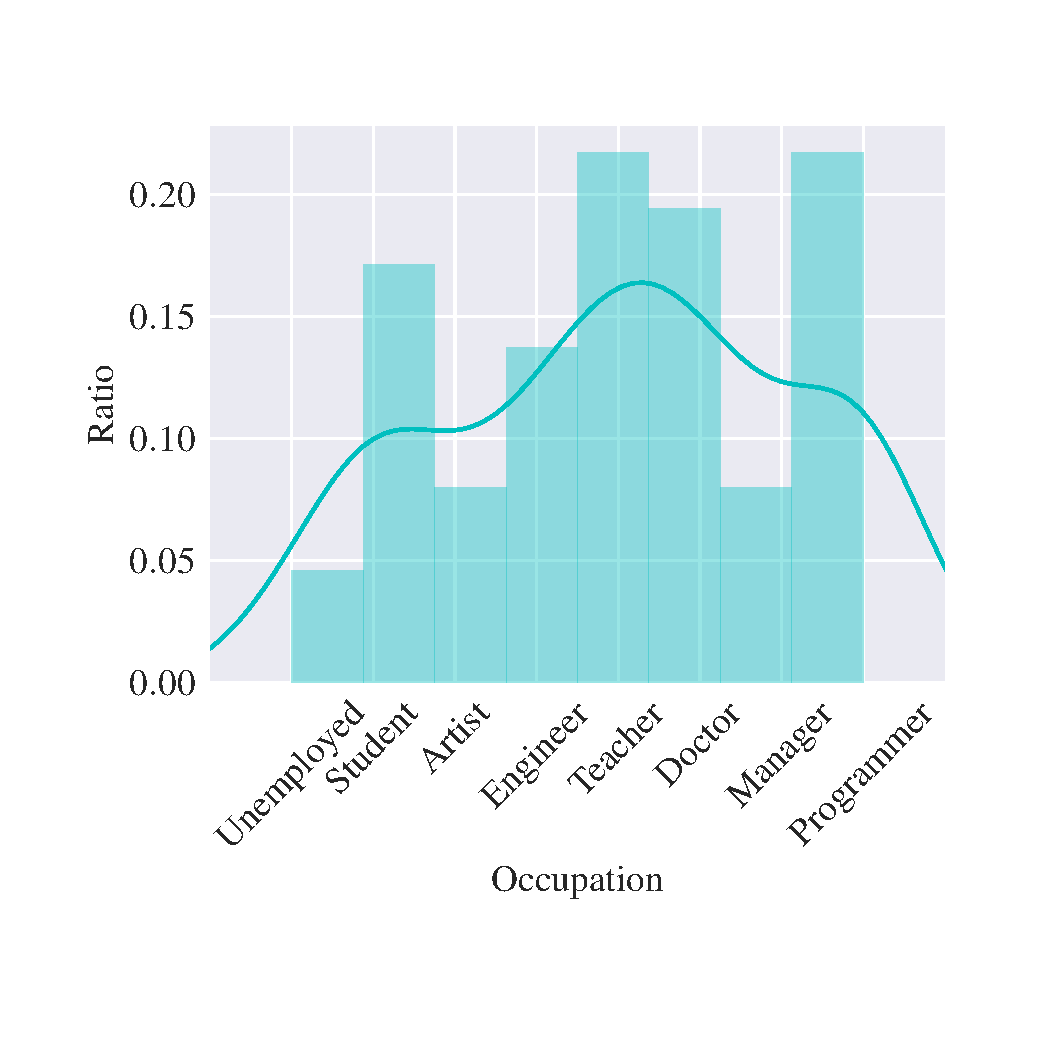
\includegraphics[width=0.31\textwidth]{fig/occup.pdf}
        \label{fig:occupation_distribution}
    }
    \subfigure[Education Distribution]{
        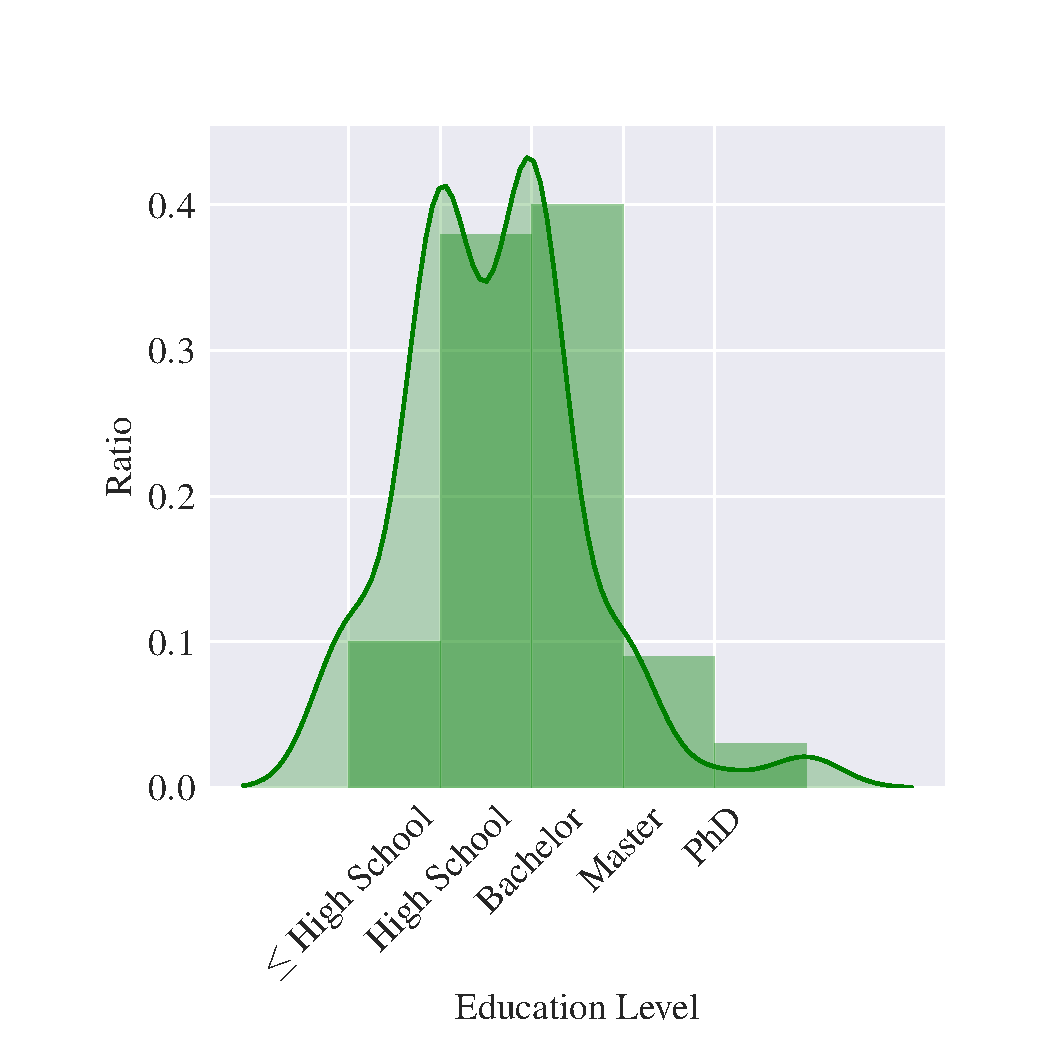
\includegraphics[width=0.31\textwidth]{fig/edu.pdf}
        \label{fig:education_distribution}
    }
    \subfigure[Education - Occupation Joint\newline Distribution]{
        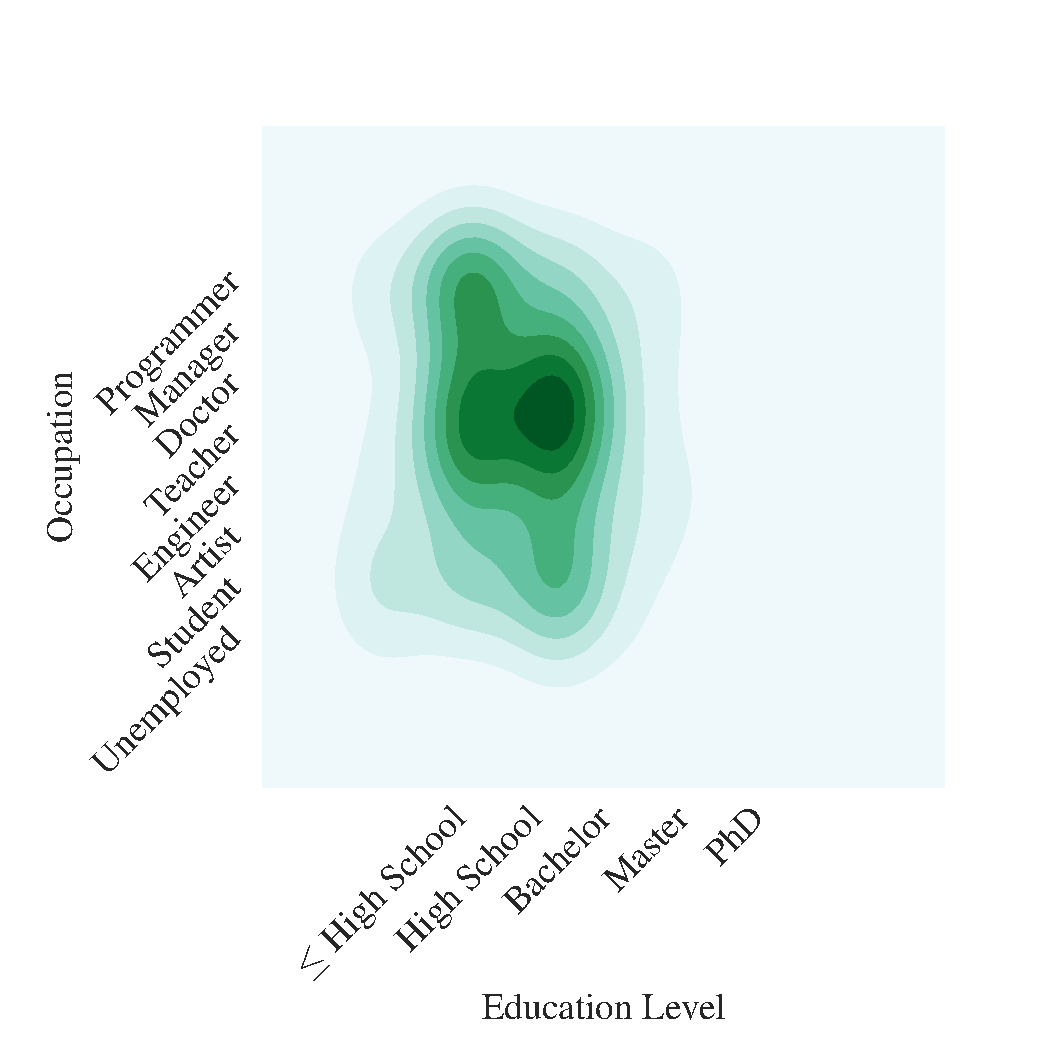
\includegraphics[width=0.31\textwidth]{fig/occu_edu.pdf}
        \label{fig:education_occupation_distribution}
    }
    \subfigure[Number of friends]{
        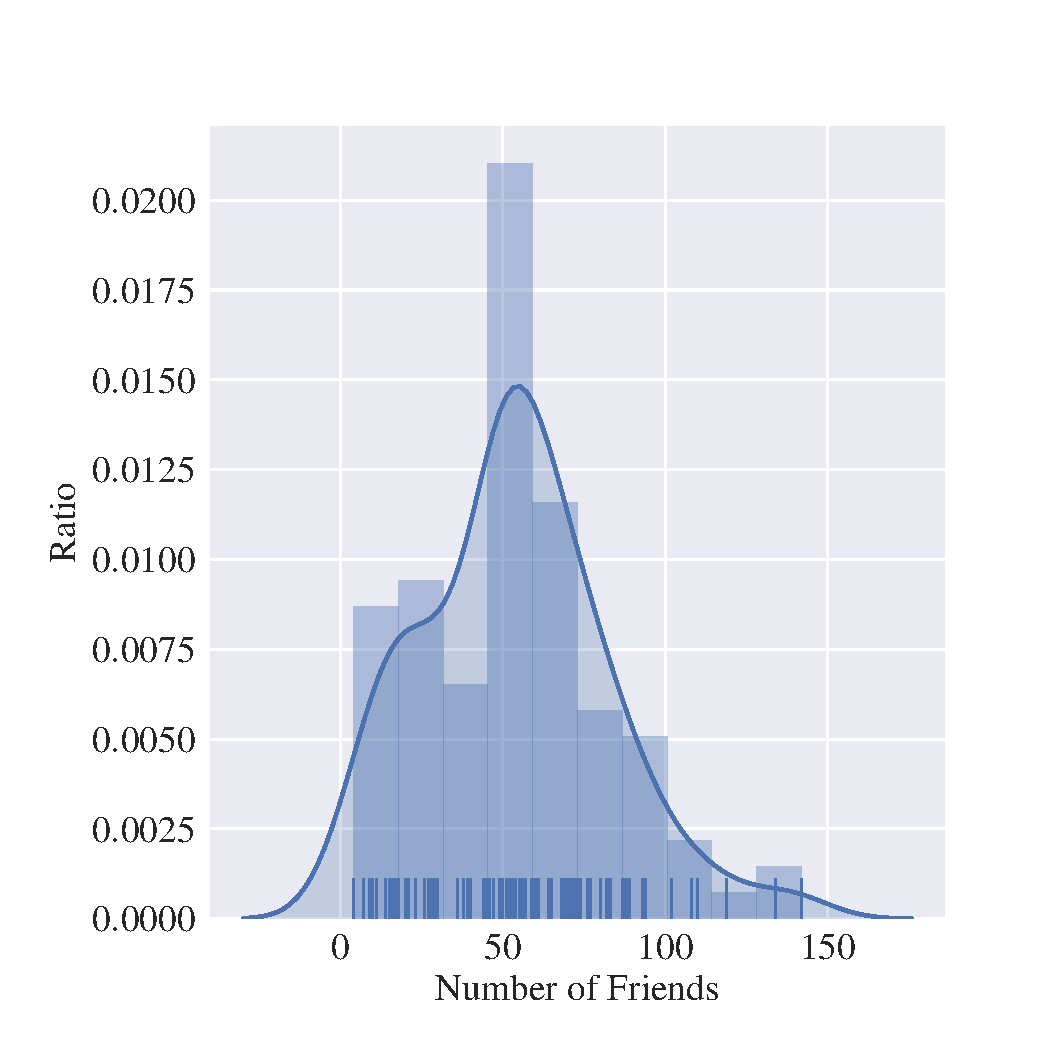
\includegraphics[width=0.31\textwidth]{fig/friends.pdf}
        \label{fig:friend_distribution}
    }
    \caption{Statistic information of \emph{PIDATA}}
    \label{fig:population_dataset}
\end{figure}

After surveying on several datasets~\cite{traud2011comparing,schwartz2013personality,pak2010twitter} and recent methods, we collect our dataset \emph{PIDATA} with an API provided by Facebook~\cite{graham2008facebook}. The usage of this dataset observes the \emph{Platform Policies}, \emph{Data Use Policy}, \emph{Statement of Rights and Responsibilities}. Corresponding statistical information is illustrated as Fig.~\ref{fig:population_dataset}. Fig~\ref{fig:age_distribution} is age distribution. Fig~\ref{fig:gender_distribution} is gender distribution. Fig~\ref{fig:education_distribution} is education distribution. Fig~\ref{fig:occupation_distribution} is occupation distribution. Fig~\ref{fig:education_occupation_distribution} is education occupation distribution. Fig~\ref{fig:friend_distribution} is friend distribution.



Fig.~\ref{fig:fvs} shows the distribution of private data over different data categories (feature vectors) of 6 selected subgroups. It is clear that the value of person's data is partially related his age and social status. Another interesting observation from Fig.~\ref{fig:fvs} is that high covariance exists between certain data categories, which will be dealt with in Sec.~\ref{sec:query_vec}.

\begin{figure}[htbp]
\begin{center}
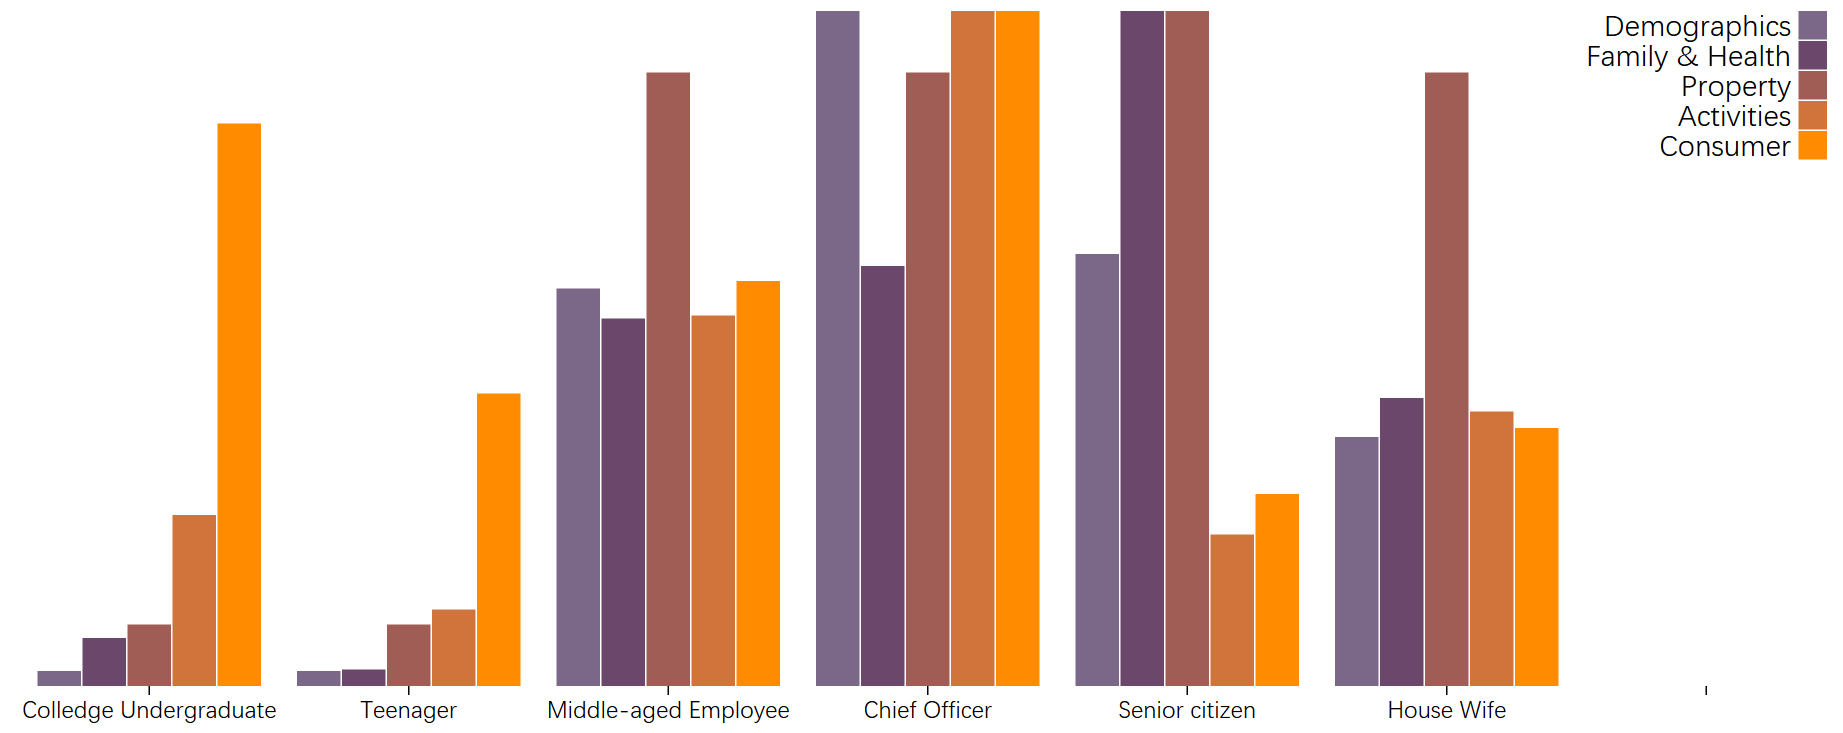
\includegraphics[width=0.85\linewidth]{fig/bars6.png}
\caption{Individual feature vectors of some typical subgroups.}
\label{fig:fvs}
\end{center}
\end{figure}

To develop a price point for PI protection, we exam the true value of a person's full data and its components. Fig.~\ref{fig:valueeee} shows how different categories of private data contributes to the value of a person's PI. 

\begin{figure}[htbp]
\begin{center}
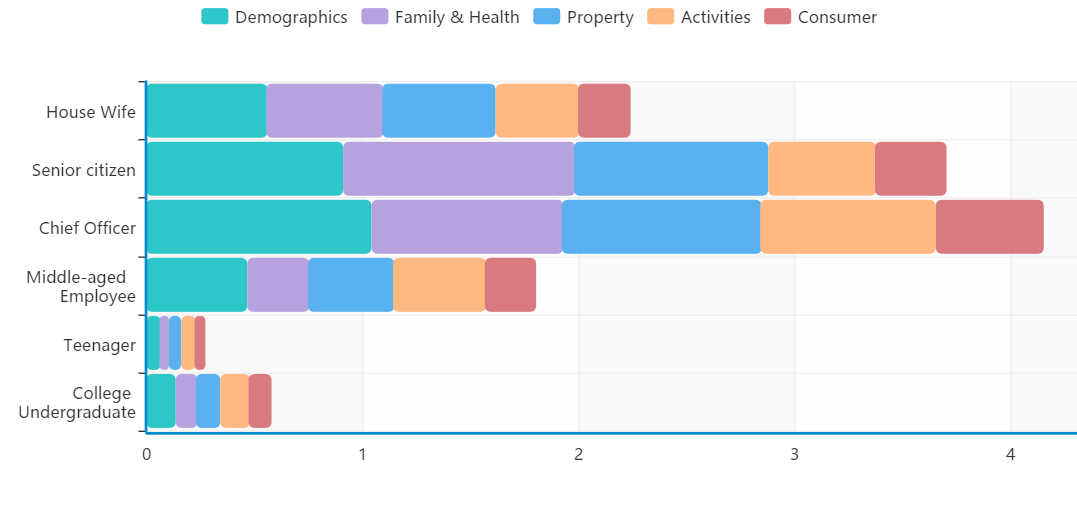
\includegraphics[width=0.85\linewidth]{fig/barr.png}
\caption{Value components of different subgroups's PI.}
\label{fig:valueeee}
\end{center}
\end{figure}

Based on the computed value of personal information, we are able to establish a price point for protecting it by treating data protection as an special insurance. Although the trade value of data can is just a few dollars, cost for each stolen data record can be as high as \$141 - roughly 70-fold of its trade value, and the likelihood of a recurring material data breach over the next two years is estimated as 27.7\%, according to a data breach study by IBM~\cite{IBMreport}. Therefore, to firmly protect a certain data record for 1 year, one must invest 10 times of its trade value calculated from Eqn.~\eqref{eqn:amend}, which leads to the deduction that it might be better to share personal data and make profits from it if the risk is low.

\subsection{Task 2: Pricing Structure of PI}
\label{sec:task2}

With the introduction of feature vectors, correlation matrix and the amendment formula (Eqn.~\eqref{eqn:amend}), we can simply determine how much a person's information is worth given a query on a specific domain. Based on a thorough survey on 77 adults, we are able to estimate the corresponding query feature vector of several query domains. The results are listed in Table~\ref{tab:qfv}. 

\begin{table}
    \centering
    \caption{Comparison between query feature vectors from various domains}
    \label{tab:qfv}
    \begin{tabular}{c c}
\hline
\specialrule{0em}{2pt}{2pt}
    	Domain & Average query feature vector\\
\specialrule{0em}{2pt}{2pt}
\hline
\specialrule{0em}{2pt}{2pt}
	Social media & $\left[\begin{matrix} 0.93 & 0.68 & 0.13 & 0.96 & 0.37 \\ \end{matrix}\right]$ \\
\specialrule{0em}{2pt}{2pt}
	Financial transactions & $\left[\begin{matrix} 0.82 & 0.53 & 0.94 & 0.24 & 0.98 \\ \end{matrix}\right]$ \\
\specialrule{0em}{2pt}{2pt}
	Health / media records & $\left[\begin{matrix} 0.26 & 0.99 & 0.08 & 0.11 & 0.10 \\ \end{matrix}\right]$ \\
\specialrule{0em}{2pt}{2pt}
	Search histories & $\left[\begin{matrix} 0.66 & 0.58 & 0.13 & 0.74 & 0.84 \\ \end{matrix}\right]$ \\
\specialrule{0em}{2pt}{2pt}
	Location info & $\left[\begin{matrix} 0.24 & 0.05 & 0.05 & 0.35 & 0.12 \\ \end{matrix}\right]$ \\
\specialrule{0em}{2pt}{2pt}
\hline
    \end{tabular}
\end{table}

Based on query feature vectors in Table~\ref{tab:qfv} and Eqn.~\eqref{eqn:value}, values of private information queried by different domains are illustrated in Fig.~\ref{fig:domains}.

\begin{figure}[htbp]
\begin{center}
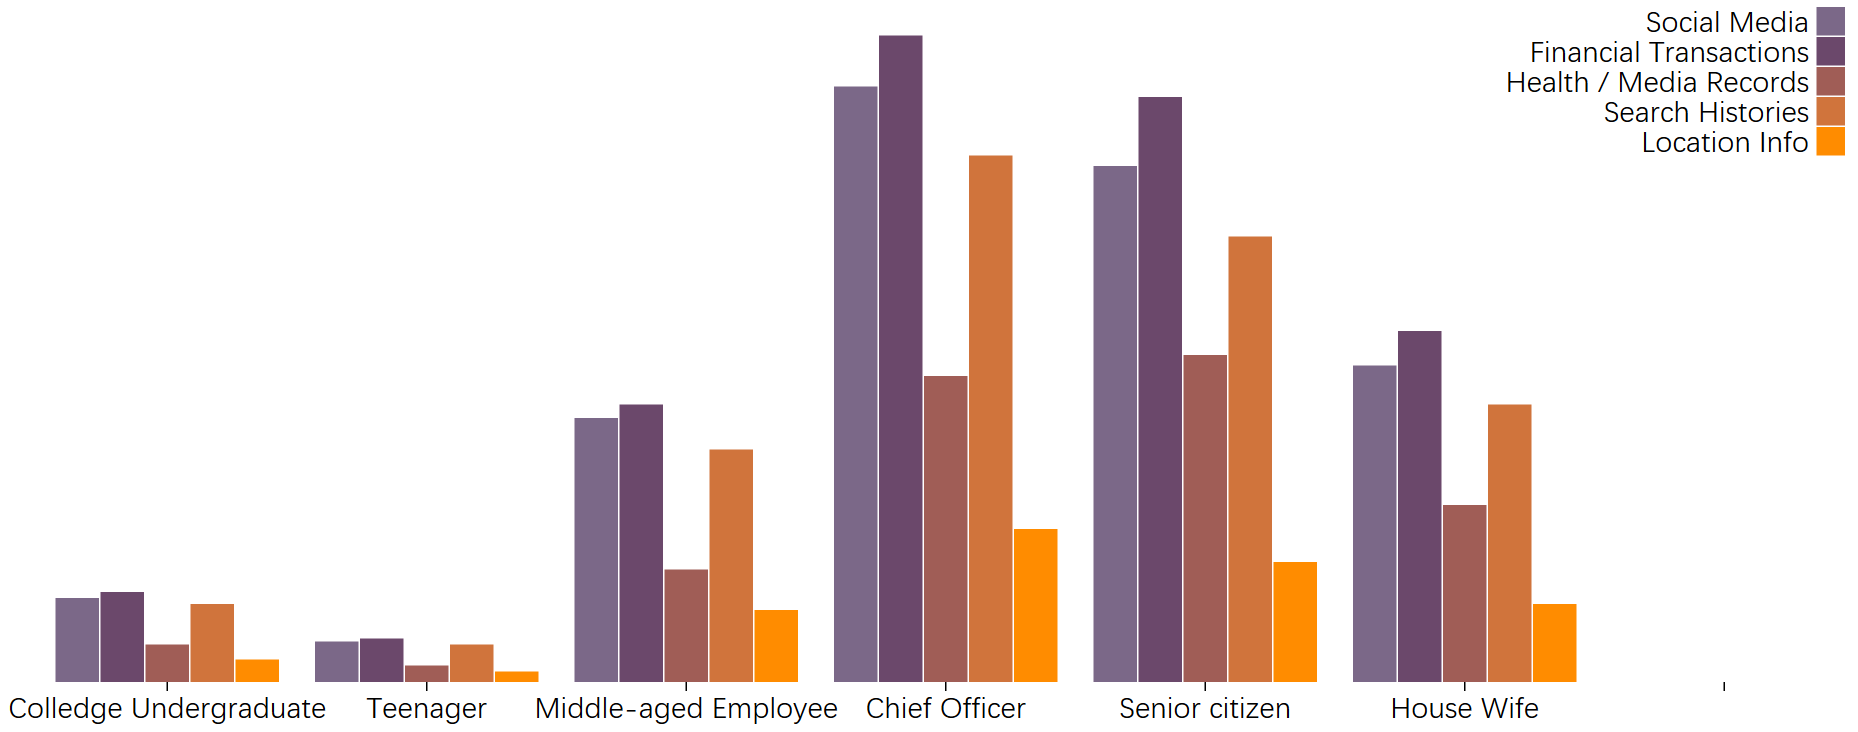
\includegraphics[width=0.85\linewidth]{fig/bar3.png}
\caption{Information value in various domains of some typical subgroups.}
\label{fig:domains}
\end{center}
\end{figure}

From results shown in Fig.~\ref{fig:domains}, we can establish a pricing structure correspondingly. The price is explicitly calculated in view of different basic elements of data via individual feature vectors defined in Sec.~\ref{sec:individual_vec}. As for cost of privacy across various domains, it can be calculated in similar manners as Sec.~\ref{task1}, where protecting cost and trade value of data are in direct proportion. If the risk of data disclosure is negligible, spending considerable money on data protection would be an unnecessary cost, and people might prefer to have their data unprotected in order to save budgets.

\subsection{Task 3: Supply and Demand}
\label{sec:task3}

People become more clear about which agencies had purchased their PI, how much their PI was worth and how PI was being used. 

Based on the above model, we evaluate the influence of the control level to the price of PI. With data becoming a commodity, we find that:
\begin{itemize}
\item It is appropriate to consider forces of supply and demand for PI. Commercial Corporations $\mathcal{Q}_1$ have higher demand for PI, which makes it possible for them to provide higher offer compared with the other two types of agencies.
\item If people have control to sell to their data, which means $\tau_j$ varies with different individuals, the price $P_{agency}$ increases with the $\tau_j$. 
\end{itemize}  

\subsection{Task 4: Assumptions and Constraints - Political/Cultural Issues}\label{sec:task4}
The assumptions and constraints of our model, which is also the political and cultural issues of the United States, European Union and other countries is listed as below. Suppose our model is proposed under the circumstance which is in compliance with local government regulations and cultural issues. Firstly, we explain the terminology used in the model.

\subsubsection{Explanation of Terminology}
\begin{itemize}
\item \textbf{Agency:} any corporations, organizations, Executive department, military department, Government corporation, Government controlled corporation, or other establishment in the executive branch of the Federal Government.
\item \textbf{Individual:} a citizen of the United States or an alien lawfully admitted for permanent residence.
\item \textbf{Private Information:} any item, collection, or grouping of information about an individual that is maintained by an agency, including, but not limited to, his education, financial transactions, medical history, and criminal or employment history and that contains his name, or the identifying number, symbol, or other identifying particular assigned to the individual, such as a finger or voice print or a photograph.
\end{itemize}

\subsubsection{Political Issues and Cultural Issues}
\textbf{The United States: \emph{Privacy Act}} \cite{act1974privacy} 

The \emph{Overview of the Privacy Act of 1974, 2015 Edition} is prepared by the Department of Justice's Office of Privacy and Civil Liberties (OPCL). Tracking the provisions of the Act itself, the Overview provides reference to and legal analysis of court decisions interpreting the Act's provisions.

The purpose of the \emph{Privacy Act} is to balance the government's need to maintain information about individuals with the rights of individuals to be protected against unwarranted invasions of their privacy stemming from federal agencies' collection, maintenance, use, and disclosure of personal information about them. More details are in the Appx.~\ref{app:privacy}.

\textbf{European Union: \emph{General Data Protection Regulation (GDPR)} \cite{regulation2016regulation}  } 

The GDPR aims primarily to give control back to citizens and residents over their personal data and to simplify the regulatory environment for international business by unifying the regulation within the EU. The regulation was adopted on $27$ April $2016$. It becomes enforceable from $25$ May $2018$ after a two-year transition period.

\underline{Data breaches.}
Under the GDPR, the Data Controller will be under a legal obligation to notify the Supervisory Authority (SA) without undue delay. The reporting of a data breach is not subject to any \emph{de minimis} standard and must be reported to the Supervisory Authority within 72 hours after having become aware of the data breach. 
%Individuals have to be notified if adverse impact is determined. In addition, the data processor will have to notify the controller without undue delay after becoming aware of a personal data breach.

% However, the notice to data subjects is not required if the data controller has implemented appropriate technical and organizational protection measures that render the personal data unintelligible to any person who is not authorized to access it, such as encryption.

% \paragraph{EU Digital Single Market.}
% The EU Digital Single Market strategy aims to open up digital opportunities for people and business and enhance Europe's position as a world leader in the digital economy. As part of this strategy the GDPR and the \emph{Directive on Security of Network and Information Systems (NIS Directive)} shall all apply from 25 May 2018. The proposed \emph{ePrivacy Regulation} is also planned to be applicable from 25 May 2018. The \emph{eIDAS Regulation} is also part of the strategy.

\underline{Citizen Control of Personal Data.}
Under the GDPR, organizations are encouraged to give back control of personal data to the individual, or citizen. %Making it easier for them to access the data organizations hold on them and for them to be able to change the permissions they grant for it to be used or shared. \emph{Personal Information Management} helps organizations give back this control, and there are a number of tools and solutions to assist with this.

\textbf{Canada: \emph{Personal Information Protection and Electronic Documents Act}} 

\textbf{The Personal Information Protection and Electronic Documents Act} (PIPEDA or the PIPED Act) is a Canadian law relating to data privacy. It governs how private sector organizations collect, use and disclose personal information in the course of commercial business. In addition, the Act contains various provisions to facilitate the use of electronic documents. 
%PIPEDA became law on 13 April 2000 to promote consumer trust in electronic commerce. The act was also intended to reassure the European Union that the Canadian privacy law was adequate to protect the personal information of European citizens. "Personal Information", as specified in PIPEDA, is as follows: information about an identifiable individual, but does not include the name, title or business address or telephone number of an employee of an organization.

The law gives individuals the right to
\begin{itemize}
\item know why an organization collects, uses or discloses their personal information;
% \item expect an organization to collect, use or disclose their personal information reasonably and appropriately, and not use the information for any purpose other than that to which they have consented;
\item know who in the organization is responsible for protecting their personal information;
\item expect an organization to protect their personal information by taking appropriate security measures;
% \item expect the personal information an organization holds about them to be accurate, complete and up-to-date;
\item obtain access to their personal information and ask for corrections if necessary; and
% \item complain about how an organization handles their personal information if they feel their privacy rights have not been respected.
\end{itemize}

% The law requires organizations to
% \begin{itemize}
% \item obtain consent when they collect, use or disclose their personal information;
% \item supply an individual with a product or a service even if they refuse consent for the collection, use or disclosure of your personal information unless that information is essential to the transaction;
% \item collect information by fair and lawful means; and
% have personal information policies that are clear, understandable and readily available.
% \end{itemize}

% cultural characteristics of information privacy.

\textbf{Japan: \emph{Act on Protection of Personal Information (APPI)}} 

APPI reflects the Japanese socio-cultural characteristics  for personal information protection. Personal information leakage cases and social responses in Japan reflect three Japanese
socio-cultural characteristics: Uchi/Soto awareness, insular collectivism and Hon'ne/Tatemae
tradition. An effective law protecting personal information in Japan's cultural environment cannot
be made simply by copying the privacy protection laws in western nations. Instead, legal protection of
personal information should be drafted that reflects and takes into account these socio-cultural
characteristics \cite{orito2008socio}.

%Japanese social customs are complex and dynamic, and often depend, and change, based on circumstance, social standing, age, professional position, and myriad other considerations. The dichotomy of honne-tatamae - the concept of a public face and a true face - is one expression of this duality. The duality of uchi-soto is another. In Japanese, Uchi literally means home, while Soto  refers to outside. The core concept of  Uchi/Soto revolves around the idea of dividing people into two groups, a in-group and an out-group.

% In April 2005, \emph{the Act on Protection of Personal Information - APPI} was enacted in Japan in response to Directive 95/46/EC. The Act was intended
% to protect personal information collected, stored, distributed, and used by both public
% and private organisations. APPI stipulates conditions of proper personal information
% handling in organisations in the private sector and is simultaneously a basic law for
% protecting personal information; the APPI held by Administrative Organs (Act No. 58
% of 2003) and the APPI held by Independent Administrative Institutions (Act No. 59 of
% 2003) were enacted under APPI and the local governments established their ordinances
% for personal information protection based on APPI. While the Act for Protection of
% Computer Processed Personal Data held by Administrative Organs (Act No. 95 of 1988)
% went into effect in 1989, a personal information protection law governing the private
% sector had not been enacted and enforced until the enactment of the APPI, mainly
% because of political pressure from Japan's business community. For example, the
% Japanese Federation of Economic Organisations (Nippon Keidanren, 2003), one of the
% strongest lobbying groups in Japan, had asserted that self-regulation was the most
% efficient means of protecting personal information in the private sector to avoid
% negative impacts on the business activities of Japanese firms.
% However, APPI has not been effective in preventing breaches of privacy; many
% incidents of personal information leakage have occurred since the Act became law. We
% have observed several cases in which such sensitive personal information as criminal
% records, medical records and prisoner's records were leaked. Evidently, a majority of
% private and public organisations seem unable to provide effective protection of personal
% information they own and use, despite explicit privacy policies announcing compliance
% with APPI, or the relevant acts or ordinances established on the basis of the Act, on their
% web sites.
\subsubsection{Price Regulations}
Generally, the data value of people varies from different regions. It's common to see quite a lot of variation by location. Fig.~\ref{fig:datavalue} is the statistical result, which is a comparison of the total number of a person's data value for countries around the world (ones without enough data are left gray) \cite{gkatzelis2015pricing}:
\begin{figure}
\begin{center}
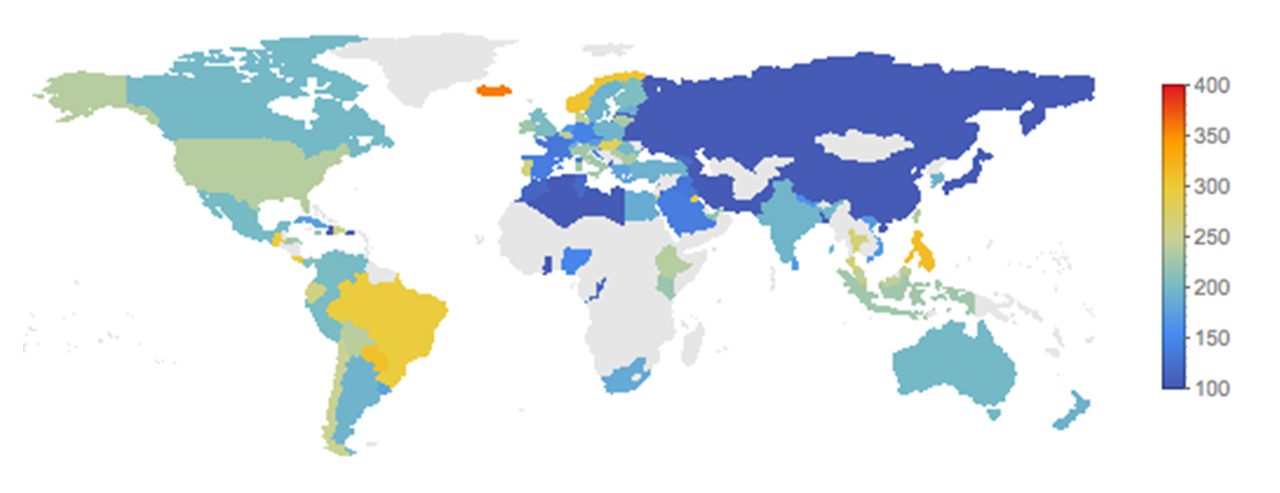
\includegraphics[width=0.9\linewidth]{fig/geoplot.png}
\caption{Data Value by locations: comparisons of the total number of a person's data value for countries around the world (ones without enough data are left gray)}
\label{fig:datavalue}
\end{center}
\end{figure}





Based on the model and the political/cultural issues, we can draw the conclusion that information privacy should be made a basic human right when thinking about policy recommendations.

\subsection{Task 5: Generation Difference}

In the perspective of risk-to-benefit ratio of PI and data privacy, there are generational differences. For example, the risk-to-benefit ratio is different between old people and young people when their health record is leaked. For old people, it is usually much higher than that of young people. 

As generation changes, the input individual attributes change and data value depends on the generation correspondingly. As for the risk-to-benefit factor we defined in Eqn.~\eqref{eqn:risk to benefit}, it describes the risk-to-benefit ratio of PI. The factor will change since the benefit score and risk score will change.  Considering all the effects that generation change have, our final data price will be affected in the process above. 
\begin{figure}
    \centering
    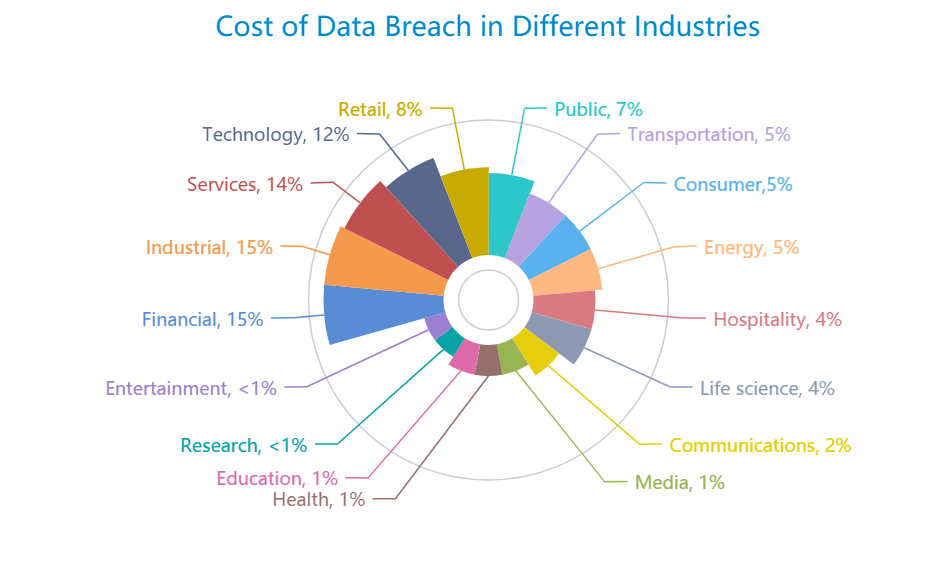
\includegraphics[width=0.8\textwidth]{fig/cost-of-industry.png}
    \caption{Cost of Data Breach in Different Industries}
    \label{fig:breach-industry}
\end{figure}
PI (private information) is different from PP (private personal property) and IP (intellectual property). PI is an abstract concept. It is non-entity. However PP often refers to the property of people. It physically exists. IP is the property of human intellect including copyrights and patents. PI is only known by the owner but IP is not only known by the owner. People all know the owner of the IP.

PI is also similar with PP and IP to some extent. PI and PP are both private while PI and PP are both abstract.

\subsection{Task 6: \emph{mCAF}: a Multi-dimensional Clustering Algorithm for Friends of Social Network Services}

Based on the \emph{mCAF} model we proposed previously, we have the following conclusions:
\begin{itemize}
\item Network effects of data sharing sharing do effect the price system for individuals, subgroups, and entire communities and nations.
\item It is the responsibility of the communities to protect citizen's PI if communities have shared privacy risks.
\end{itemize}


\subsection{Task 7: Data Breach Effect}
Data breach, especially massive data breach where millions of prople's PI are stolen will affect the privacy a lot. Taking TJX data breach as example, it involves more than 100 million records and causes 118 million dollars loss to cover the loss and potential liabilities. That does not include the loss in reputation of brand and other indirect cost. From the research of IBM~\cite{IBMreport}, we get cost of data breach for different industries (Fig.~\ref{fig:breach-industry}) and countries (Fig.~\ref{fig:breach-region}). We can see that data breach widely exists and PI loss is a factor that we should not neglect.

\begin{figure}
    \centering
    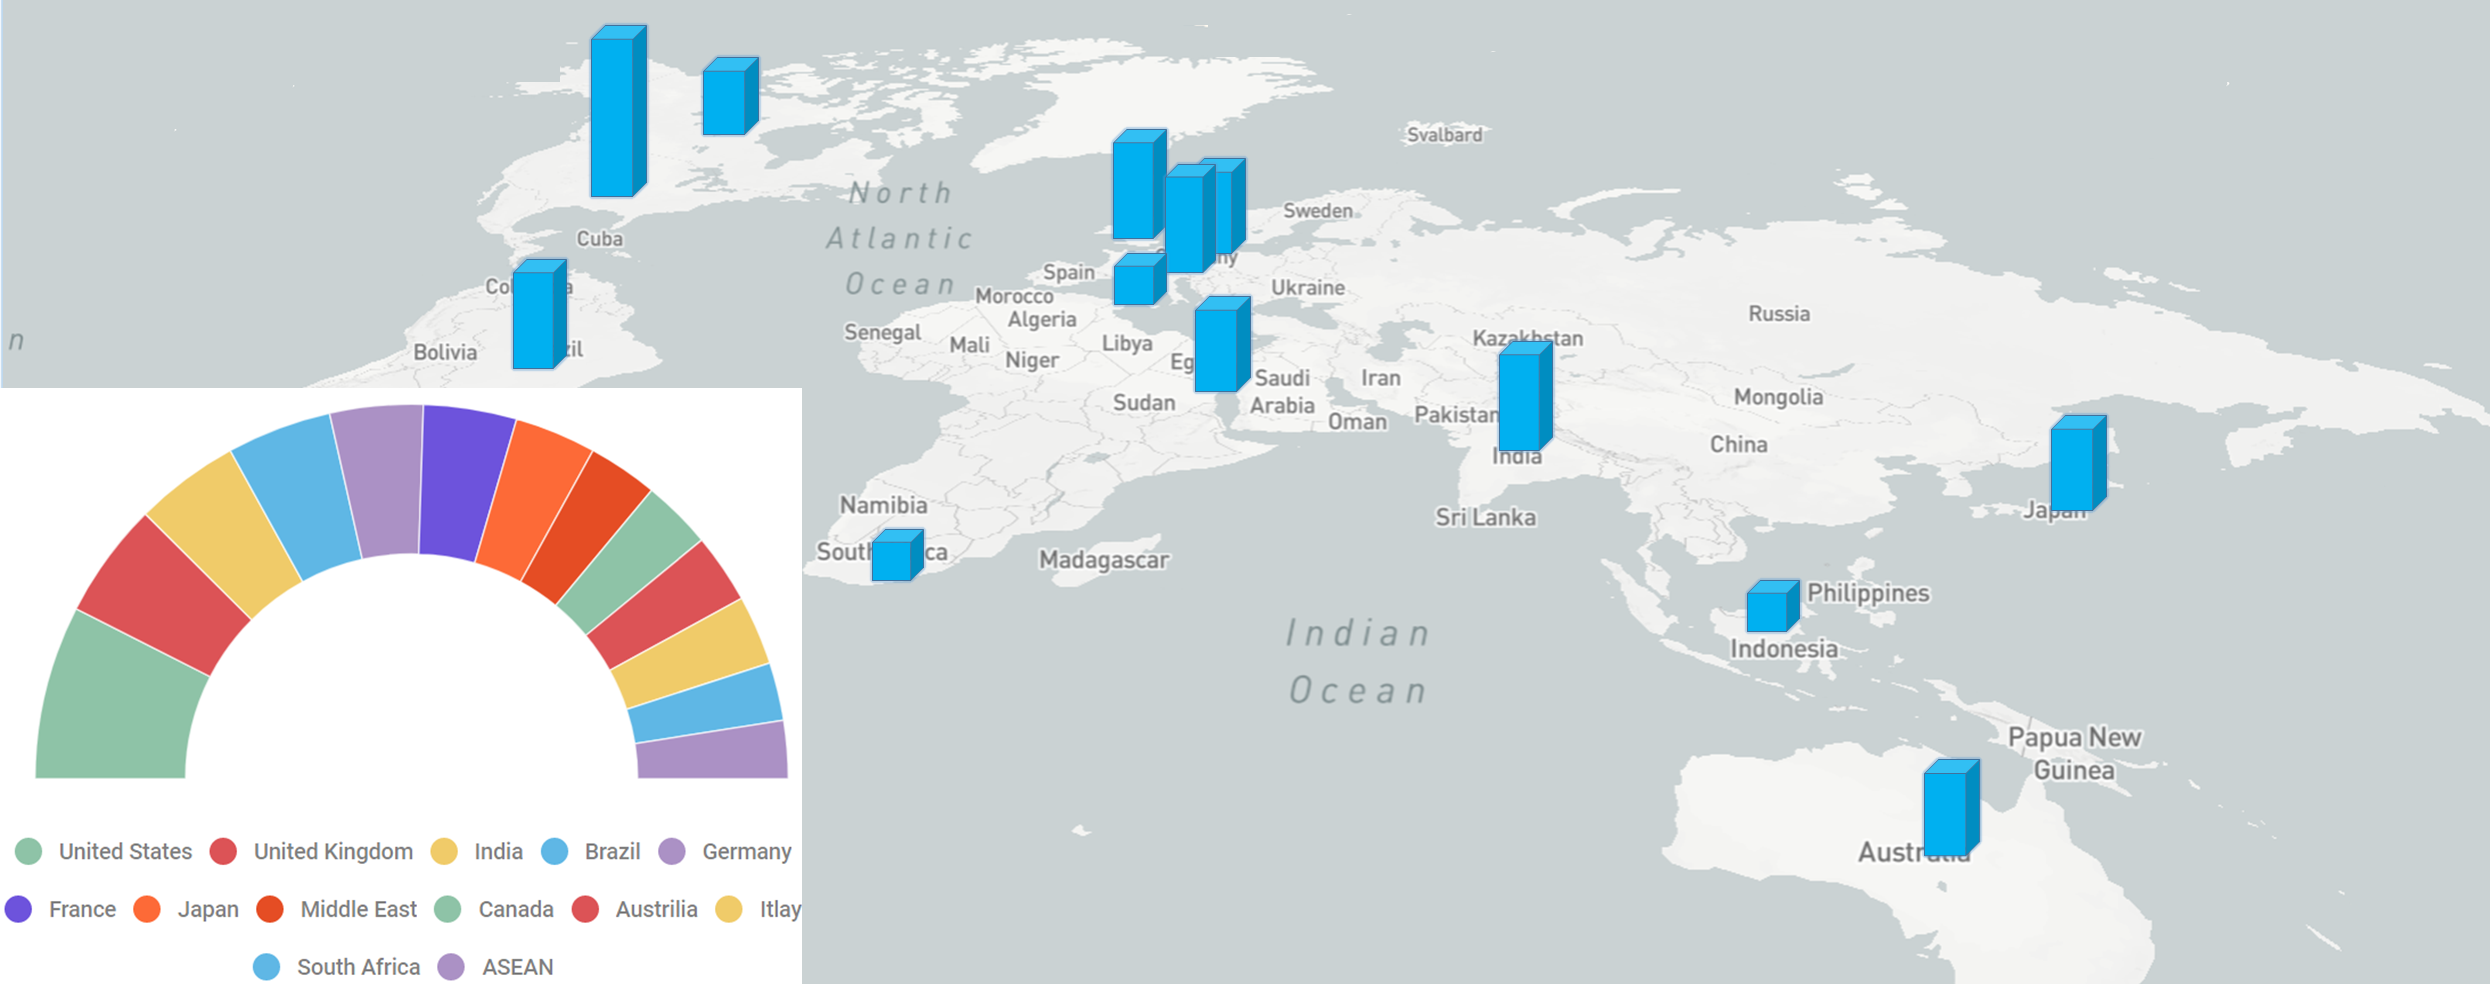
\includegraphics[width=\textwidth]{fig/map.png}
    \caption{Cost of Data Breach in Different Regions}
    \label{fig:breach-region}
\end{figure}

The PI loss and cascade event caused by massive data breach will impact the price point. In our model, we have considered such effect. Eqn.~\eqref{equ:demand model} shows the trade off between the price and data breach effect. When massive data breach happens, the trade off factor $\lambda_j$ will be smaller and thus $\lambda_j p_j$ will be smaller. $r_j$ depends on the level of data breach. For massive data breach and the corresponding cascade event, it would be higher. We can see that the price will be lower. It is reasonable since data breach will violate the assumption that all the gathered data are managed by a trusted third-party organization, which protects users' data and helps sell them under owner's permission. People's data will be sold without permission or even be used as ransom. Some PI buyers will buy the breach data in an illegal way instead of buying data from people or trusted third-party organization. Demand will decrease and the price will be lower.

Agencies that breach the data should be responsible for the data breach and pay the individuals directly. As shown above, price of data will be much lower after massive data breach happens. The agencies should be responsible for the PI loss even if they don't intend to breach the data.

\section{Sensitivity Analysis}

In this part we will do sensitivity analysis on our model. The sensitivity analysis show that our model is generalized and performs stably under different conditions, by which we are convinced that our model is able to solve the problem successfully.

\subsection{Demand Model} This part shows the PI purchasers are sensitive to price and illustrates how it is possible to identify heterogeneous price sensitivities in the data. This heterogeneity will play a key role when we later use the model to study the equilibrium effects of the PI's price restrictions, because this heterogeneity affects which types of purchasers change their purchasing behavior in response to different relative price changes.

The event-time-specific estimates is shown as Eqn.~\eqref{equ:Qjt}:
\begin{equation}\label{equ:Qjt}
\log Q_{jt}=\alpha_j+\alpha_t+\beta_j t+\alpha_{A,t}+\epsilon_{jt},
\end{equation}
where $Q_{jt}$ denotes retention rates among existing buyers for data provider $j$ at time $t$. The first two $\alpha$ terms in this equation implement a standard difference-in-difference design, while the $\alpha_{A,t}$ terms capture differences between data provider $A$ and other. For sake of presentation, the $\beta$ term is included to account for different time trends among the included data providers.
When estimating the demand side of the model, we use price variation to estimate heterogeneous price sensitivities across different purchaser types. 

\subsection{\emph{mCAF} Model}
We adopt the multi-dimensional clustering algorithm for friends (\emph{mCAF}) to perform identify social clusters. mCAF algorithm  randomizes the center points initially. We run mCAF several times on our dataset \emph{PIDATA} and analyze the result. 

We propose a metric to evaluate the sensitivity of mCAF in Eqn.~\eqref{eqn:metric}, where $Eq(\cdot)$ is defined in Eqn.~\eqref{eqn:eqfunction}

\begin{equation}\label{eqn:metric}
\delta= \frac{\sum_{i\in V} Eq(l_i,l_{0_i})}{\sum_{i\in V} 1}
\end{equation}

\begin{equation}\label{eqn:eqfunction}
Eq(x,y)= \left\{\begin{array}{ll}
1 &\mbox{if } x \ne \mbox{ y}\\
0 &\mbox{otherwise}.
\end{array}\right.
\end{equation}

Table~\ref{tab:result} shows the results from 8 experiments, from which we can conclude that the $\delta$ is very small in all experiments. It proofs that mCAF model perfoms well and is robust under different situations. 

\begin{table}[!htbp]
    \centering
    \caption{Result of Sensitivity Analysis on mCAF }
    \label{tab:result}
    \begin{tabularx}{\textwidth}{X X X X X X X X X  }
\hline
\specialrule{0em}{2pt}{2pt}
    $Exp No$ & 1&2&3&4&5&6&7&8\\
    \hline
\specialrule{0em}{2pt}{2pt}
 $\delta$ & 0.025&0.013&0.025&0.013&0.051&0.013&0.013&0.025\\
\specialrule{0em}{2pt}{2pt}
\hline
    \end{tabularx}
\end{table}

\section{Conclusions and Future Work}
We develop a complete pricing system that accurately estimates the intrinsic value as well as market price of a certain individual's data under a specific query request. Out method consists of three core components: a value calculator that maps a query and an individual to value of that data, a dynamic market system to further compute its market price, and a social cluster model to estimate the network effect on data price. In the environments and sensitivity analysis of our model, we find that it is accurate and generalized enough to be adopted in a wide range of domains.

One limitation of our current approach is that our model requires a large dataset to precisely estimate the correlation matrix as well as many other parameters used in its mechanism. A promising future direction is to combine out methods with better estimation algorithms, e.g. Analytic Hierarchy Process (AHP), to reduce the variance caused by insufficient data.

In future work, our goal is to introduce non-linear data value predictors, e.g. neural networks, to characterize a more complicated relationship between individuals and data. Additionally, we plan to extend the current dataset in both scale and coverage to cater to the needs of deep learning algorithms.

% Private information will continue to increase dramatically in both quality and diversity, and has the potential to unlock significant economic and societal value.

% Based on our model, we can draw the conclusion that:
% \begin{itemize}

% \item Invest in open and collaborative trials orchestrated by end user privacy groups or academics;
% \item Integrate principles surrounding and user trust and data protection into the development of new services and platforms;
% \item Engage with leading innovators and end user advocacy groups to explore the further applications for, and development of, trust framework;
% \item Policy makers and agencies should launch an international dialog, which should encompass governments, international bodies such as the World Trade Organization, end user privacy rights groups and representation from the private sector. It should include not only US and European Union members, but interested parties from the Asia-Pacific region and emerging countries;
% \item For the United States: Agencies  should closely watch developments of the National Stategy for Trusted Identities in Cyberspace program and the privacy bill - and seek ways to contribute to them. Agencies need to be in constant dialog with the US Department of Commerce, the Federal Trade Commission and other bodies to help shape future legislation and policies;
% \item For the European Union: Agencies should collaborate with the European Commission in its move to revise the EU privacy directive and to synchronize legislation across its member states. 
% \item For other countries: In other regions that differ from the US or the EU in cultural or social norms, very different paths in adopting policy frameworks will be required. However, given the global relevance of many such markets in the future data economy, agencies and policy makers should not just wait and see. One initial step in making progress could be to seek ways to harmonize fragmented national privacy policies.
% \end{itemize}

	\bibliographystyle{IEEEtran}
	\bibliography{newrefs}
	
\begin{appendix}


\section{Implementation of Function $\sigma(\cdot)$}
\label{appx:sigma}

We format our $\langle attribute, value \rangle$ database in the form of a reader-friendly questionnaire consisting of five parts, each corresponding to a data category as value vectors in our database concentrate values in one dimension. The five scores generated by the following questionnaire make up for the five elements in the individual feature vector of the tester.

\subsection{Demographics}

\begin{table}[H]
    \centering
    \begin{tabularx}{0.8\textwidth}{X p{2cm}}
\hline
\specialrule{0em}{2pt}{2pt}
    Has the following information been leaked? &Value\\
\specialrule{0em}{2pt}{2pt}
\hline
\specialrule{0em}{2pt}{2pt}
	Age & \$0.0005\\
\specialrule{0em}{2pt}{2pt}
	Gender & \$0.0005\\
\specialrule{0em}{2pt}{2pt}
	ZIP Code & \$0.0005\\
\specialrule{0em}{2pt}{2pt}
	 Ethnicity & \$0.005\\
\specialrule{0em}{2pt}{2pt}
	 Education level & \$0.0005\\
\specialrule{0em}{2pt}{2pt}
\hline
    \end{tabularx}
\end{table}

\begin{table}[H]
    \centering
    \begin{tabularx}{0.8\textwidth}{X p{2cm}}
\hline
\specialrule{0em}{2pt}{2pt}
    Are you a millionaire? &Value\\
\specialrule{0em}{2pt}{2pt}
\hline
\specialrule{0em}{2pt}{2pt}
Yes & \$0.116\\
\specialrule{0em}{2pt}{2pt}
No & \$0\\
\specialrule{0em}{2pt}{2pt}
\hline
    \end{tabularx}
\end{table}

\begin{table}[H]
    \centering
    \begin{tabularx}{0.8\textwidth}{X p{2cm}}
\hline
\specialrule{0em}{2pt}{2pt}
    Are you engaged to be married? If so, how long? &Value\\
\specialrule{0em}{2pt}{2pt}
\hline
\specialrule{0em}{2pt}{2pt}
Yes, one month or less & \$0.12\\
\specialrule{0em}{2pt}{2pt}
Yes, one to three months & \$0.115\\
\specialrule{0em}{2pt}{2pt}
Yes, more than three months & \$0.10\\
\specialrule{0em}{2pt}{2pt}
No & \$0\\
\specialrule{0em}{2pt}{2pt}
\hline
    \end{tabularx}
\end{table}

\begin{table}[H]
    \centering
    \begin{tabularx}{0.8\textwidth}{X p{2cm}}
\hline
\specialrule{0em}{2pt}{2pt}
    Are you? &Value\\
\specialrule{0em}{2pt}{2pt}
\hline
\specialrule{0em}{2pt}{2pt}
Recently married? & \$0.01\\
\specialrule{0em}{2pt}{2pt}
Recently divorced? & \$0.01\\
\specialrule{0em}{2pt}{2pt}
Empty nester? & \$0.01\\
\specialrule{0em}{2pt}{2pt}
\hline
    \end{tabularx}
\end{table}

\begin{table}[H]
    \centering
    \begin{tabularx}{0.8\textwidth}{X p{2cm}}
\hline
\specialrule{0em}{2pt}{2pt}
   What is your job? &Value\\
\specialrule{0em}{2pt}{2pt}
\hline
\specialrule{0em}{2pt}{2pt}
Accountant & \$0.072\\
\specialrule{0em}{2pt}{2pt}
Altorney & \$0.08\\
\specialrule{0em}{2pt}{2pt}
Banking and finance executive & \$0.08\\
\specialrule{0em}{2pt}{2pt}
Chairman & \$0.076\\
\specialrule{0em}{2pt}{2pt}
Chief executive & \$0.086\\
\specialrule{0em}{2pt}{2pt}
Chief financial officer & \$0.086\\
\specialrule{0em}{2pt}{2pt}
Chief information officer & \$0.086\\
\specialrule{0em}{2pt}{2pt}
Chief operating officer & \$0.086\\
\specialrule{0em}{2pt}{2pt}
Chief technology officer & \$0.086\\
\specialrule{0em}{2pt}{2pt}
Company owner & \$0.086\\
\specialrule{0em}{2pt}{2pt}
Cosmetologist+Beauty & \$0.072\\
\specialrule{0em}{2pt}{2pt}
Entrepreneur & \$0.10\\
\specialrule{0em}{2pt}{2pt}
Health professional & \$0.072\\
\specialrule{0em}{2pt}{2pt}
Human resources executive & \$0.08\\
\specialrule{0em}{2pt}{2pt}
Home improvement contractor & \$0.072\\
\specialrule{0em}{2pt}{2pt}
Insurance agent & \$0.072\\
\specialrule{0em}{2pt}{2pt}
Licensed professional & \$0.072\\
\specialrule{0em}{2pt}{2pt}
Manufacturing \& Engineering & \$0.072\\
\specialrule{0em}{2pt}{2pt}
Non-profit & \$0.072\\
\specialrule{0em}{2pt}{2pt}
Pilot & \$0.072\\
\specialrule{0em}{2pt}{2pt}
Pharmaceutical industry exec & \$0.076\\
\specialrule{0em}{2pt}{2pt}
President & \$0.086\\
\specialrule{0em}{2pt}{2pt}
Real estate agent or broker & \$0.072\\
\specialrule{0em}{2pt}{2pt}
Vice chairman & \$0.086\\
\specialrule{0em}{2pt}{2pt}
Other & \$0\\
\specialrule{0em}{2pt}{2pt}
\hline
    \end{tabularx}
\end{table}

\subsection{Family \& Health}
\begin{table}[H]
    \centering
    \begin{tabularx}{0.8\textwidth}{X p{2cm}}
\hline
\specialrule{0em}{2pt}{2pt}
    Do you have children? &Value\\
\specialrule{0em}{2pt}{2pt}
\hline
\specialrule{0em}{2pt}{2pt}
Yes & \$0.005\\
\specialrule{0em}{2pt}{2pt}
No & \$0\\
\specialrule{0em}{2pt}{2pt}
\hline
    \end{tabularx}
\end{table}

\begin{table}[H]
    \centering
    \begin{tabularx}{0.8\textwidth}{X p{2cm}}
\hline
\specialrule{0em}{2pt}{2pt}
    Are you expecting a baby? If so, will this be your first childand which  trimester are you in? &Value\\
\specialrule{0em}{2pt}{2pt}
\hline
\specialrule{0em}{2pt}{2pt}
Yes Yes First & \$0.095\\
\specialrule{0em}{2pt}{2pt}
Yes Yes Second & \$0.115\\
\specialrule{0em}{2pt}{2pt}
Yes Yes Third & \$0.115\\
\specialrule{0em}{2pt}{2pt}
Yes No First & \$0.08\\
\specialrule{0em}{2pt}{2pt}
Yes No Second & \$0.10\\
\specialrule{0em}{2pt}{2pt}
Yes No Third & \$0.10\\
\specialrule{0em}{2pt}{2pt}
No & \$0\\
\specialrule{0em}{2pt}{2pt}
\hline
    \end{tabularx}
\end{table}

\begin{table}[H]
    \centering
    \begin{tabularx}{0.8\textwidth}{X p{2cm}}
\hline
\specialrule{0em}{2pt}{2pt}
   Are you a new parent? If so, is your new baby a boy or girl?  &Value\\
\specialrule{0em}{2pt}{2pt}
\hline
\specialrule{0em}{2pt}{2pt}
Yes Boy & \$0.035\\
\specialrule{0em}{2pt}{2pt}
Yes Girl  & \$0.035\\
\specialrule{0em}{2pt}{2pt}
No & \$0\\
\specialrule{0em}{2pt}{2pt}
\hline
    \end{tabularx}
\end{table}

\begin{table}[H]
    \centering
    \begin{tabularx}{0.8\textwidth}{X p{2cm}}
\hline
\specialrule{0em}{2pt}{2pt}
   Do you have any of the following conditions? &Value\\
\specialrule{0em}{2pt}{2pt}
\hline
\specialrule{0em}{2pt}{2pt}
 Acid reflux & \$0.26\\
 \specialrule{0em}{2pt}{2pt}
    ADHD & \$0.26\\
  \specialrule{0em}{2pt}{2pt}
    Allergies & \$0.26\\
     \specialrule{0em}{2pt}{2pt}
   Arthritis & \$0.26\\
     \specialrule{0em}{2pt}{2pt}
   Asthma & \$0.26\\
     \specialrule{0em}{2pt}{2pt}
   Back pain & \$0.26\\
     \specialrule{0em}{2pt}{2pt}
   Clinical depression & \$0.26\\
     \specialrule{0em}{2pt}{2pt}
    Diabetes & \$0.26\\
     \specialrule{0em}{2pt}{2pt}
    Frequent heartburn & \$0.26\\
     \specialrule{0em}{2pt}{2pt}
    Headaches/migraines & \$0.26\\
\specialrule{0em}{2pt}{2pt}
\hline
    \end{tabularx}
\end{table}

\subsection{Property}
\begin{table}[H]
    \centering
    \begin{tabularx}{0.8\textwidth}{X p{2cm}}
\hline
\specialrule{0em}{2pt}{2pt}
   Do you own a home? &Value\\
\specialrule{0em}{2pt}{2pt}
\hline
\specialrule{0em}{2pt}{2pt}
Yes & \$0.085\\
     \specialrule{0em}{2pt}{2pt}
  No & \$0\\
\specialrule{0em}{2pt}{2pt}
\hline
    \end{tabularx}
\end{table}

\begin{table}[H]
    \centering
    \begin{tabularx}{0.8\textwidth}{X p{2cm}}
\hline
\specialrule{0em}{2pt}{2pt}
   If you own a home, it is likely that data companies already know this information about you from public databases: &Value\\
\specialrule{0em}{2pt}{2pt}
\hline
\specialrule{0em}{2pt}{2pt}
 The size of your home & \$0.005\\
     \specialrule{0em}{2pt}{2pt}
The size of your mortgage & \$0.005\\
     \specialrule{0em}{2pt}{2pt} 
     How many bathrooms the property has & \$0.005\\
     \specialrule{0em}{2pt}{2pt} 
     How many bedrooms the property has & \$0.005\\
     \specialrule{0em}{2pt}{2pt}
\hline
    \end{tabularx}
\end{table}

\begin{table}[H]
    \centering
    \begin{tabularx}{0.8\textwidth}{X p{2cm}}
\hline
\specialrule{0em}{2pt}{2pt}
   If you own a home, Has the following information been released on public databases? & Value\\
\specialrule{0em}{2pt}{2pt}
\hline
\specialrule{0em}{2pt}{2pt}
Yes & \$0.085\\
     \specialrule{0em}{2pt}{2pt}
  No & \$0\\
\specialrule{0em}{2pt}{2pt}
\hline
    \end{tabularx}
\end{table}

\begin{table}[H]
    \centering
    \begin{tabularx}{0.8\textwidth}{X p{2cm}}
\hline
\specialrule{0em}{2pt}{2pt}
   Is there a fireplace in your home? &Value\\
\specialrule{0em}{2pt}{2pt}
\hline
\specialrule{0em}{2pt}{2pt}
Yes & \$0\\
     \specialrule{0em}{2pt}{2pt}
  No & \$0\\
\specialrule{0em}{2pt}{2pt}
\hline
    \end{tabularx}
\end{table}

\subsection{Activities}

\begin{table}[H]
    \centering
    \begin{tabularx}{0.8\textwidth}{X p{2cm}}
\hline
\specialrule{0em}{2pt}{2pt}
   Do you have any of these hobbies? &Value\\
\specialrule{0em}{2pt}{2pt}
\hline
\specialrule{0em}{2pt}{2pt}
 Are you a cruise enthusiast? & \$0.03\\
     \specialrule{0em}{2pt}{2pt}
       Are you a fitness and excercise buff? & \$0.03\\
     \specialrule{0em}{2pt}{2pt}
  Are you interested in foreign travel? & \$0.03\\
\specialrule{0em}{2pt}{2pt}
\hline
    \end{tabularx}
\end{table}

\begin{table}[H]
    \centering
    \begin{tabularx}{0.8\textwidth}{X p{2cm}}
\hline
\specialrule{0em}{2pt}{2pt}
  Do you own an aircraft? &Value\\
\specialrule{0em}{2pt}{2pt}
\hline
\specialrule{0em}{2pt}{2pt}
Yes & \$0.085\\
     \specialrule{0em}{2pt}{2pt}
  No & \$0\\
\specialrule{0em}{2pt}{2pt}
\hline
    \end{tabularx}
\end{table}

\begin{table}[H]
    \centering
    \begin{tabularx}{0.8\textwidth}{X p{2cm}}
\hline
\specialrule{0em}{2pt}{2pt}
Do you own a boat? &Value\\
\specialrule{0em}{2pt}{2pt}
\hline
\specialrule{0em}{2pt}{2pt}
Yes & \$0.076\\
     \specialrule{0em}{2pt}{2pt}
  No & \$0\\
\specialrule{0em}{2pt}{2pt}
\hline
    \end{tabularx}
\end{table}

\begin{table}[H]
    \centering
    \begin{tabularx}{0.8\textwidth}{X p{2cm}}
\hline
\specialrule{0em}{2pt}{2pt}
Do you exercise or participate in other activities to lose weight? &Value\\
\specialrule{0em}{2pt}{2pt}
\hline
\specialrule{0em}{2pt}{2pt}
Yes & \$0.105\\
     \specialrule{0em}{2pt}{2pt}
  No & \$0\\
\specialrule{0em}{2pt}{2pt}
\hline
    \end{tabularx}
\end{table}

\subsection{Consumer}

\begin{table}[H]
    \centering
    \begin{tabularx}{0.8\textwidth}{X p{2cm}}
\hline
\specialrule{0em}{2pt}{2pt}
Have you searched online or visited websites recently on any of these topics? (please select as many as appropriate) &Value\\
\specialrule{0em}{2pt}{2pt}
\hline
\specialrule{0em}{2pt}{2pt}
Auto & \$0.0021\\
     \specialrule{0em}{2pt}{2pt}
  Financial information & \$0.001\\
  \specialrule{0em}{2pt}{2pt}
 Retail & \$0.001\\
 \specialrule{0em}{2pt}{2pt}
 Travel& \$0.001\\
 \specialrule{0em}{2pt}{2pt}
 Gossip & \$0.0013\\
 \specialrule{0em}{2pt}{2pt}
 Gaming & \$0.0013\\
 \specialrule{0em}{2pt}{2pt}
 Food & \$0.0013\\
 \specialrule{0em}{2pt}{2pt}
Education & \$0.0013\\
 \specialrule{0em}{2pt}{2pt}
Cooking topics & \$0.0008\\
 \specialrule{0em}{2pt}{2pt}
 Movie information & \$0.003\\
 \specialrule{0em}{2pt}{2pt}
Political and govermental topics & \$0.0019\\
 \specialrule{0em}{2pt}{2pt}
Telecom and television purchase research & \$0.0015\\
\specialrule{0em}{2pt}{2pt}
\hline
    \end{tabularx}
\end{table}

\begin{table}[H]
    \centering
    \begin{tabularx}{0.8\textwidth}{X p{2cm}}
\hline
\specialrule{0em}{2pt}{2pt}
Do you hold any store loyalty cards, at a grocery store or pharmacy, for instance? &Value\\
\specialrule{0em}{2pt}{2pt}
\hline
\specialrule{0em}{2pt}{2pt}
Yes & \$0.001\\
     \specialrule{0em}{2pt}{2pt}
  No & \$0\\
\specialrule{0em}{2pt}{2pt}
\hline
    \end{tabularx}
\end{table}

\begin{table}[H]
    \centering
    \begin{tabularx}{0.8\textwidth}{X p{2cm}}
\hline
\specialrule{0em}{2pt}{2pt}
Are you looking to buy any of these products? (Select as many as appropriate) &Value\\
\specialrule{0em}{2pt}{2pt}
\hline
\specialrule{0em}{2pt}{2pt}
 Car(s) & \$0.0018\\
     \specialrule{0em}{2pt}{2pt}
   Consumer packaged goods such as soap, shampoo, toilet paper etc & \$0.001\\
\specialrule{0em}{2pt}{2pt}
Education & \$0.0013\\
     \specialrule{0em}{2pt}{2pt}
     Financial products or services & \$0.001\\
     \specialrule{0em}{2pt}{2pt}
   Other vehicles & \$0.0011\\
     \specialrule{0em}{2pt}{2pt}
       Clothes & \$0.0008\\
     \specialrule{0em}{2pt}{2pt}
      Travel & \$0.0011\\
     \specialrule{0em}{2pt}{2pt}
\hline
    \end{tabularx}
\end{table}

\begin{table}[H]
    \centering
    \begin{tabularx}{0.8\textwidth}{X p{2cm}}
\hline
\specialrule{0em}{2pt}{2pt}
Are you looking to buy a mobile phone? &Value\\
\specialrule{0em}{2pt}{2pt}
\hline
\specialrule{0em}{2pt}{2pt}
Yes & \$0.0125\\
     \specialrule{0em}{2pt}{2pt}
  No & \$0\\
\specialrule{0em}{2pt}{2pt}
\hline
    \end{tabularx}
\end{table}

\section{Privacy Act}
\label{app:privacy}

In 1974, Congress was concerned with curbing the illegal surveillance and investigation of individuals by federal agencies that had been exposed during the Watergate scandal.  It was also concerned with potential abuses presented by the government's increasing use of computers to store and retrieve personal data by means of a universal identifier - such as an individual's social security number.  The Act focuses on four basic policy objectives:
\begin{itemize}
\item To restrict disclosure of personally identifiable records maintained by agencies.
\item To grant individuals increased rights of access to agency records maintained on themselves.
\item To grant individuals the right to seek amendment of agency records maintained on themselves upon a showing that the records are not accurate, relevant, timely, or complete.
\item To establish a code of "fair information practices" that requires agencies to comply with statutory norms for collection, maintenance, and dissemination of records.
\end{itemize}


\end{appendix}
%\newpage
%\section*{Executive Summary}
	
%\noindent To whom it may concern,
	
%\newpage

%\begin{appendices}

%\section{Implemented Genetic Algorithm}
%\lstinputlisting[language=Matlab]{gene.m}
%\section{Fitness Function}
%\lstinputlisting[language=Matlab]{fitness.m}
%\end{appendices}
\end{document}